% +--------------------------------------------------------------------+
% | LaTeX Template for K-State Electronic Theses, Dissertations,
% | and Reports
% |
% | Some guidelines for using the template are shown in comments.  Read
% | these comments carefully, as they describe changes you will need to
% | make to the template in order to meet Graduate School requirements.            |
% |
% | Additional information on using the template are contained in these
% | files, which are included when you download the template:
% |
% | ReadMe.pdf - A general overview of using the template
% |
% | BibTeX Guide.pdf - Detailed guidelines on using BibTeX to create
% | your bibliography and manage your citations.
% |
% | natbib.pdf - Gives detailed information on using the natbib package
% | and formatting citations
% +--------------------------------------------------------------------+

% +--------------------------------------------------------------------+
% | The template is designed to be used with PDFLaTeX. Process this
% | file (etdrtemplate.tex) with PDFLaTeX in order to produce a PDF
% | version of your ETDR.  If you are using BibTex to manage your
% | refrences, you will need to process your file four times:
% | 1. Run PDFLaTeX
% | 2. Run BibTex
% | 3. Run PDFLaTeX
% | 4. Run PDFLaTeX
% |
% | Some LaTeX editors do not explicitly list PDFLaTeX as an option, but
% | do use PDFLaTeX to produce a PDF file directly from your .tex files.
% | See the ReadMe file for details.
% +--------------------------------------------------------------------+
% |
% +--------------------------------------------------------------------+
% |
% | As required by the Graduate School, The template is configured to
% | contain the following sections in the order shown.

% | Abstract title page (doctoral dissertations only)
% | Abstract (doctoral dissertations only)
% | Title page
% | Copyright page
% | Abstract
% | Table of contents
% | List of figures
% | List of tables
% | Acknowledgements (Optional)
% | Dedication (Optional)
% | Preface (Optional)
% | Individual Chapters
% | References or Bibliography
% | Appendices (as needed)
% |
% | Details on removing optional sections are given in the comments below.
% |
% +--------------------------------------------------------------------+

% +--------------------------------------------------------------------+
% | The LaTex command \documentclass selects a particular class to
% | associate with the document.  Within this command, 12pt is
% | specified for the font size.  You can change this to 11 pt, if
% | desired.
% +--------------------------------------------------------------------+

\documentclass[final,letterpaper,12pt,oneside]{tex/styles/class_diss}

% +--------------------------------------------------------------------+
% | Here are added external packages that will be used throughout
% | the document.  You can add other packages as needed.
% +--------------------------------------------------------------------+

\usepackage{graphicx} % Extended graphics package.
\usepackage{booktabs} % nice rules (thick lines) for tables
\usepackage{tabulary}
\usepackage{microtype} % improves typography for PDF
\usepackage{xcolor} % Allows color
\usepackage{amsmath} % American Mathematics Society standards
\usepackage{amsxtra} % Additional math symbols
\usepackage{amssymb} % Additional math symbols
\usepackage{amsthm} % Additional math symbols
\usepackage{latexsym} % Additional math symbols
\usepackage{setspace} % Controls line spacing
\usepackage[margin=1in]{geometry} % Sets page margins to 1 inch on all sides
\usepackage[titles]{tocloft} % Adds leader dots to all entries in the table of contents
\usepackage{bm}
\usepackage{tikz}
\usepackage{verbatim}
\usepackage{braket}
\usepackage{longtable}
\usepackage[parfill]{parskip}
\usepackage{standalone}
\usepackage[ruled,vlined]{algorithm2e}


% +--------------------------------------------------------------------+
% | put your own definitions here
% +--------------------------------------------------------------------+

\newcommand{\SN}{S$_N$}
\renewcommand{\vec}[1]{\bm{#1}} %vector is bold italic
\newcommand{\vd}{\bm{\cdot}} % slightly bold vector dot
\newcommand{\grad}{\vec{\nabla}} % gradient
\newcommand{\ud}{\mathop{}\!\mathrm{d}} % upright derivative symbol
\newcommand{\oper}[1]{\mathcal{#1}}
\providecommand{\e}[1]{\ensuremath{\times 10^{#1}}}
\newcommand{\CHAPTER}[1]{Chapter~\ref{#1}} 
\newcommand{\EQ}[1]{Eq.~(\ref{#1})}               %-- Eq. (refeq)
\newcommand{\EQUATION}[1]{Equation~(\ref{#1})}    %-- Equation (refeq)
\newcommand{\FIG}[1]{Fig.~\ref{#1}}               %-- Fig. refig
\newcommand{\FIGURE}[1]{Figure~\ref{#1}} 
\newcommand{\TAB}[1]{Table~\ref{#1}}              %-- Table tablref
\newcommand{\EQS}[2]{Eqs.~(\ref{#1})--(\ref{#2})}            %-- Eqs. (refeqs)
\newcommand{\EQUATIONS}[2]{Equations~(\ref{#1})--(\ref{#2})}   %-- Eqs. (refeqs)
\newcommand{\EQSTWO}[2]{Eqs.~(\ref{#1})~and~(\ref{#2})}     %-- Eqs. (refeqs)
\newcommand{\EQUATIONSTWO}[2]{Equations~(\ref{#1})~and~(\ref{#2})} 

% +--------------------------------------------------------------------+
% |
% | Citation and Bibliography Style
% |
% | The following commands determine the citation and bibliography style.  The
% | template uses BibTeX for formatting the bibliography.  See "BibTeX Guide.pdf"
% | for details on formatting citations and references.  The template is set
% | to use a generic, superscript style, but it can be easily modified
% | to use author-year styles.

\bibliographystyle{unsrtnat}
% | If you want to use an author-year citation style, change "unsrtnat" to
% | "plainnat" in the line above.  You can also use other styles supported
% | by LaTeX, e.g., acm, ieeetr, siam, etc.  Additional styles
% | are in the \styles folder and can be invoked like this:
% | \bibliographystyle{styles/apsrev}.  If the style you use is based
% | on an author-year citation style, you will need to make changes
% | in the usepackage and \setcitestyle statements below

\usepackage[super,sort&compress]{natbib}
% | If you want to use an author-year citation style, change "super" to
% | "authoryear" in the line above.

\setcitestyle{super}
% | if you want to use an author-year citation style, change "super" to
% | "authoryear" in the line above.

% +---------------------------------------------------------------------+
% | The hyperref package enables cross-references.
% +---------------------------------------------------------------------+

\usepackage[pdftex, plainpages=false, pdfpagelabels]{hyperref}

\hypersetup{
    linktocpage=true,
    colorlinks=true,
    bookmarks=true,
    citecolor=blue,
    urlcolor=blue,
    linkcolor=blue,
    citebordercolor={1 0 0},
    urlbordercolor={1 0 0},
    linkbordercolor={.7 .8 .8},
    breaklinks=true,
    pdfpagelabels=true,
    }

% +--------------------------------------------------------------------+
% | The document begins here.
% +--------------------------------------------------------------------+

\doublespacing
\begin{document}

% +--------------------------------------------------------------------+
% | ******Masters Students -- You Need to Make Some Changes Here******
% |
% | The Abstract Title page and Abstract page following the Abstract
% | Title page are required only for doctoral dissertations.  For
% | masters theses or reports, comment out or delete the lines:
% |
% | % +--------------------------------------------------------------------+
% | Abstract Title Page
% |
% |This page is required only for doctoral dissertations.
% +--------------------------------------------------------------------+

% +--------------------------------------------------------------------+
% | This page should not contain a page number.  We use the
% | \thispagestyle[empty] command below to suppress page numbers
% | and other style elements.
% +--------------------------------------------------------------------+

\thispagestyle{empty}

% +--------------------------------------------------------------------+
% | The Abstract Title page begins here
% +--------------------------------------------------------------------+

\pdfbookmark[0]{Title Page}{PDFTitlePage}
%\setcounter{page}{1}

\begin{center}

   \vspace{1cm}

% +--------------------------------------------------------------------+
% | Enter the title of your ETDR below.  For 2017 and on, use "Sentence case" (not ALL CAPS).
% | For details, see:  k-state.edu/grad/etdr/create/sentencecase.html 
% +--------------------------------------------------------------------+

   \large Enter your title in sentence case\\

   \vspace{0.5cm}

   by\\

   \vspace{0.5cm}

% +--------------------------------------------------------------------+
% | Enter your name below in standard name format (not ALL CAPS).
% +--------------------------------------------------------------------+

   \large Enter Your Name\\

   \vspace{0.5cm}

% +--------------------------------------------------------------------+
% | On the line below, replace "Enter Your Previous Degrees"
% | with your previous degrees in mixed case. Include the abbreviation
% | for the degree, the name of the university, and the year separated
% | by commas. For example:
% |
% |    B.A., University of Illinois, 2000
% |
% | If desired, it is acceptable to include a city or country with
% | the university name. For example:
% |
% |    B.S., Jillian University, China, 2002
% |
% | Each degree should appear on a separate line.  Use the \\
% | command to create a line break.
% +--------------------------------------------------------------------+

   Enter Your Previous Degrees\\

   \vspace{0.55cm}
   \rule{2in}{0.5pt}\\
   \vspace{0.75cm}

   {\large AN ABSTRACT OF A DISSERTATION}\\

   \vspace{0.5cm}
   \begin{singlespace}
   submitted in partial fulfillment of the\\
   requirements for the degree\\
   \end{singlespace}

   \vspace{0.5cm}

% +--------------------------------------------------------------------+
% | On the line below, enter the name of your earned degree in ALL
% | CAPITAL LETTERS.  For example: DOCTOR OF PHILOSOPHY
% +--------------------------------------------------------------------+


   {\large ENTER YOUR DEGREE NAME}\\
   \vspace{0.5cm}

% +--------------------------------------------------------------------+
% | On the two lines below, enter the name of your department and the
% | name of the college in mixed case.  For example:
% |
% |     Biochemistry Department
% |     College of Arts and Sciences
% +--------------------------------------------------------------------+

   \begin{singlespace}
   Enter Your Department Name\\
   Enter Your College Name\\
   \end{singlespace}

   \vspace{0.5cm}

   \begin{singlespace}
   {\Large KANSAS STATE UNIVERSITY}\\
   Manhattan, Kansas\\
   \end{singlespace}

% +--------------------------------------------------------------------+
% | On the line below, replace "Graduation Year" with the four-digit year
% | of your graduation. For example:
% |
% |     2017
% +--------------------------------------------------------------------+

   Graduation Year\\
   \vspace{1cm}

\end{center}
 through \end{abstract}.
% |
% | You will also need to uncomment the two lines following the
% | \begin{abstract} command:
% |    %\setcounter{page}{-1}
% |    %\pdfbookmark[0]{Abstract}{PDFAbstractPage}
% |
% | Don't uncomment the lines above.  Scroll down several lines until
% | you see the section "For masters theses or reports, uncomment
% | the commands..." and uncomment the lines in that section.
% +--------------------- ----------------------------------------------+


% +--------------------------------------------------------------------+
% | Title Page -- Required for both Doctoral and Masters Students
% +--------------------------------------------------------------------+

% +--------------------------------------------------------------------+
% | Title Page
% +--------------------------------------------------------------------+

\newpage

% +--------------------------------------------------------------------+
% | This page should not contain a page number.  We use the
% | \thispagestyle[empty] command below to suppress page numbers
% | and other style elements.
% +--------------------------------------------------------------------+

\thispagestyle{empty}

% +--------------------------------------------------------------------+
% | The Title page begins here.
% +--------------------------------------------------------------------+

\begin{center}

   \vspace{1cm}

% +--------------------------------------------------------------------+
% | Enter the title of your ETDR below. For 2017 and on, use "Sentence case" (not ALL CAPS).
% | For details, see: k-state.edu/grad/etdr/create/sentencecase.html 
% +--------------------------------------------------------------------+

\large Origami, Lounge Chairs and Other Topics in Unfolding\\

\vspace{0.5cm}

by\\

\vspace{0.5cm}

% +--------------------------------------------------------------------+
% | Enter your name below in standard name format (not ALL CAPS).
% +--------------------------------------------------------------------+

\large John Charles Boyington\\

 \vspace{0.3cm}

% +--------------------------------------------------------------------+
% | On the line below, replace "Enter Your Previous Degrees"
% | with your previous degrees in mixed case. Include the abbreviation
% | for the degree, the name of the university, and the year separated
% | by commas. For example:
% |
% |    B.A., University of Illinois, 2000
% |
% | If desired, it is acceptable to include a city or country with
% | the university name. For example:
% |
% |    B.S., Jillian University, China, 2002
% |
% | Each degree should appear on a separate line.  Use the \\
% | command to create a line break.
% +--------------------------------------------------------------------+

   B.S., Kansas State University, 2016\\

   \vspace{0.35cm}
   \rule{2in}{0.5pt}\\
   \vspace{0.65cm}

   {\large A THESIS}\\

   \vspace{0.3cm}
   \begin{singlespace}
   submitted in partial fulfillment of the\\
   requirements for the degree\\
   \end{singlespace}

   \vspace{0.3cm}

% +--------------------------------------------------------------------+
% | On the line below, replace "ENTER YOUR DEGREE NAME" with the name
% | of your earned degree in ALL CAPITAL LETTERS.
% +--------------------------------------------------------------------+

   {\large MASTER OF SCIENCE}\\
   \vspace{0.3cm}

% +--------------------------------------------------------------------+
% | On the two lines below, replace "Enter Your Department Name" and
% | "Enter Your College Name" with the name of your department and the
% | name of the college in mixed case.  For example:
% |
% |     Biochemistry Department
% |     College of Arts and Sciences
% +--------------------------------------------------------------------+

   \begin{singlespace}
   Department of Mechanical and Nuclear Engineering\\
   College of Engineering\\
   \end{singlespace}

   \vspace{0.3cm}

   \begin{singlespace}
   {\large KANSAS STATE UNIVERSITY}\\
   Manhattan, Kansas\\
   \end{singlespace}

% +--------------------------------------------------------------------+
% | On the line below, replace "Graduation Year" with the four-digit
% | year of your graduation.  For example:
% |
% |     2016
% +--------------------------------------------------------------------+

   2019\\
   \vspace{0.3cm}

    \end{center}

    \begin{flushright}
    Approved by:\\
    \vspace{0.3cm}
    \begin{singlespace}
    Major Professor


% +--------------------------------------------------------------------+
% | On the line below, replace "Enter Your Major Professor's Name"
% | with  the name of your major professor in mixed case.  Use the
% | format Firstname Lastname.  For example:
% |
% |     Lori Goetsch
% |
% +--------------------------------------------------------------------+

    Jeremy Roberts\\
    \end{singlespace}
    \end{flushright}

% +--------------------------------------------------------------------+
% | If you have co-major professors, comment out the lines above from
% | \begin{flushright} through \end{flushright} and uncomment the
% | lines below.  Enter your co-major professors' names where indicated.
% +--------------------------------------------------------------------+

%\begin{flushright}
%   Approved by:\\
%  \vspace{ 0.3cm}
%   \begin{singlespace}
%   Co-Major Professor\\
%   Enter Your Co-Major Professor's Name\\
%   \vspace{.25cm}
%   Co-Major Professor\\
%   Enter Your Co-Major Professor's Name\\
%   \end{singlespace}
%\end{flushright}


% +--------------------------------------------------------------------+
% | Copyright Page -- Required for both Doctoral and Masters Students
% +--------------------------------------------------------------------+

% +--------------------------------------------------------------------+
% | Copyright Page
% +--------------------------------------------------------------------+

\newpage

\thispagestyle{empty}

\vspace*{0.9cm}

\begin{center}

{\bf \Huge Copyright}

\vspace{1cm}

% +--------------------------------------------------------------------+
% | The Graduate School is using a new 1-line format for 2017 and on, with 
% | the copyright symbol, author name, graduation year and a period at the end.
% | On the line below, replace "Enter Your Name" with your name.
% | Use the same form of your name as it appears on your title page, and 
% |   use mixed case (no more ALL CAPS).  For example:  Barack Obama
% | Replace "YYYY" with the four-digit year of your graduation.  
% | Be sure to include the period  after the year.  
% | EXAMPLE:  © Will E. Wildcat 2017.
% +--------------------------------------------------------------------+

   \Large\copyright\  Leidong Xu 2019.\\

   \vspace{0.5cm}


\end{center}



% +--------------------------------------------------------------------+
% |  Abstract -- Required for both Doctoral and Masters Students
% +--------------------------------------------------------------------+

\begin{abstract}

% +--------------------------------------------------------------------+
% | For masters theses or reports, uncomment the commands on the next
% | two lines (\setcounter and \pdfbookmark)
% +--------------------------------------------------------------------+

\setcounter{page}{-1}
\pdfbookmark[0]{Abstract}{PDFAbstractPage}

% +--------------------------------------------------------------------+
% | Abstract Page
% +--------------------------------------------------------------------+

\pagestyle{empty}
%\vspace{1cm}
\setlength{\baselineskip}{0.8cm}

%\indent

% +--------------------------------------------------------------------+
% | Enter the text of your abstract below.  There is no limit on the
% | number of words in your abstract.
% +--------------------------------------------------------------------+

An algorithm based on dynamic mode decomposition (DMD) is presented for acceleration of the power method (PM) and flattened power method (FPM), which takes advantage of prediction from a restarted DMD process to correct an unconverged solution.
The power method is a simple iterative scheme for determining the dominant eigenmode, and its variants, such as flattened power method, have been used to solve the of k-eigenvalue problem in reactor analysis.
DMD is a data driven technique that extracts dynamics information from time-series data with which a reduced-order surrogate model can be constructed.
DMD-accelerated PM (DMD-PM) and DMD-accelerated FPM (DMD-FPM) generate ``snapshots'' from a few iterations and extrapolatein ``fictitious time'' to estimate of a more accurate eigenvector from the dominant mode.  
This process is repeated until the solution is converged within a suitable tolerance.

To illustrate the performance of both two schemes, a 1-D test problem designed to resemble a boiling water reactor (BWR) and the well-studied 2-D C5G7 benchmark were analyzed.
Compared to the PM without acceleration, these tests have demonstrated that DMD-PM and DMD-FPM method can reduce the number of iterations significantly.



\vfill
\end{abstract}

% +--------------------------------------------------------------------+
% | The following commands start a new page and set the page numbering
% | to lowercase roman numerals.
% +--------------------------------------------------------------------+

\newpage
\pagenumbering{roman}

% +--------------------------------------------------------------------+
% |
% | *********************** IMPORTANT ******************************
% |
% | In the \setcounter command below, set the number to represent the
% | page number of the table of contents page.  For example, if the
% | table of contents page is the 6th page of your document, enter 6
% | in the brackets.  This number may vary, depending on the length of
% | your abstract.
% |
% | Numbers do not appear on the title and abstract pages, but they
% | are included in the page count.  The table of contents page is the
% | first page on which page numbers are displayed.
% +--------------------------------------------------------------------+

\setcounter{page}{6}

% +--------------------------------------------------------------------+
% | The following command creates a bookmark for the table of contents
% | in the final PDF document.
% +--------------------------------------------------------------------+

\pdfbookmark[0]{\contentsname}{contents}

% +--------------------------------------------------------=-----------+
% | The following command adds dot leaders for all entries in the
% | table of contents.
% +--------------------------------------------------------------------+

\renewcommand{\cftchapleader}{\cftdotfill{\cftdotsep}}

% +--------------------------------------------------------------------+
% | The following commands makes all entries and page numbers in the
% | table of contents appear in normal weight font (not bold).
% +--------------------------------------------------------------------+

\renewcommand{\cftchapfont}{\mdseries}
\renewcommand{\cftchappagefont}{\mdseries}

% +--------------------------------------------------------------------+
% | These commands add the table of contents, list of figures, and
% | list of tables.
% +--------------------------------------------------------------------+

\tableofcontents
\listoffigures
\listoftables

% +--------------------------------------------------------------------+
% | Symbols Page
% +--------------------------------------------------------------------+

%\phantomsection
%\addcontentsline{toc}{chapter}{List of Symbols}
%% +--------------------------------------------------------------------+
% | Title Page
% +--------------------------------------------------------------------+

\newpage

\vspace*{0.9cm}
\begin{center}
{\bf \Huge List of Symbols}
\end{center}

% +--------------------------------------------------------------------+
% | This page should not contain a page number.  We use the
% | \thispagestyle[empty] command below to suppress page numbers
% | and other style elements.
% +--------------------------------------------------------------------+

\thispagestyle{empty}

% +--------------------------------------------------------------------+
% | The Symbols page begins here.
% +--------------------------------------------------------------------+

\begin{center}
\begin{longtable}{lll}

\multicolumn{1}{c}{\textbf{Symbol}} & \multicolumn{1}{c}{\textbf{Description}} & \multicolumn{1}{c}{\textbf{Units}} \\ \hline 
\endfirsthead

\multicolumn{3}{c}%
{{\bfseries -- continued from previous page}} \\
\multicolumn{1}{c}{\textbf{Symbol}} &
\multicolumn{1}{c}{\textbf{Description}} &
\multicolumn{1}{c}{\textbf{Unit}} \\ \hline 
\endhead

\multicolumn{3}{r}{{Continued on next page}} \\
\endfoot

\endlastfoot

$\nabla$ & del operator &  \\

\end{longtable}
\end{center}


% +--------------------------------------------------------------------+
% | Acknowledgements Page
% |
% | If you choose not to have an Acknowledgements page, comment out
% | or delete the following 3 lines.
% +--------------------------------------------------------------------+

\newpage
\phantomsection
\addcontentsline{toc}{chapter}{Acknowledgements}
% +--------------------------------------------------------------------+
% | Acknowledgements Page (Optional)
% +--------------------------------------------------------------------+

\newpage
\vspace*{0.9cm}
\begin{center}
{\bf \Huge Acknowledgments}
\end{center}

\setlength{\baselineskip}{0.8cm}

%\pdfbookmark[0]{Acknowledgements}{PDF_Acknowledgements}

% +--------------------------------------------------------------------+
% | Enter text for your acknowledgements in the space below this box.
% |                                                                    
% +--------------------------------------------------------------------+
I would take some time to thank who has helped me at K-State.

First, I thank my parents, Xu Fajian and Lv Wei, who works as two distinguished mechanical engineers and pushed me to this great field.

I would like to thank to my advisor Professor Jeremy Roberts for providing me this great opportunity working on this project. He has served as my both undergraduate and graduate advisor with considerable patience since 2014.

I would like to thank Professor James Chen for leading me to numerical mathematics and encourage in me to challenge myself.   

I would like to thank Professors Mingjun Wei and Hitesh Bindra for serving on my thesis committee and for answering any of my questions.

I would also like to thank two mentors and great friends, Dr.~Mohammad Abdo and Richard Reed, for teaching me a great amount of expertise in nuclear engineering and data science.

I sincerely appreciate the help from my friends and colleagues at K-State - Cheikh, Dr. Wenkai Fu, Dr. Luis Wonnell, Khalid, Mohsen, Rabab, John, and Ye.

For the funding for this effort, I acknowledge the Alan Levin Department of Mechanical and Nuclear Engineering department for sponsoring me in the past two years. 

% +--------------------------------------------------------------------+
% | Dedication Page
% |
% | If you choose not to have a Dedication page, comment out
% | or delete the following 3 lines.
% +--------------------------------------------------------------------+

\newpage
\phantomsection
\addcontentsline{toc}{chapter}{Dedication}
% +--------------------------------------------------------------------+
% | Dedication Page (Optional)
% +--------------------------------------------------------------------+

\newpage
\vspace*{0.9cm}
\begin{center}
{\bf \Huge Dedication}
\end{center}

\setlength{\baselineskip}{0.8cm}

%\pdfbookmark[0]{Dedication}{PDF_Dedication}

% +--------------------------------------------------------------------+
% | Enter the text for your dedication in the space below this box.    
% +--------------------------------------------------------------------+

Enter the text for your Dedication page in the dedication.tex file.
The Dedication page is optional.  If you wish to remove it, see the
comments in the etdrtemplate.tex file.


% +--------------------------------------------------------------------+
% | Preface Page
% |
% | If you choose not to have a Dedication page, comment out
% | or delete the following 4 lines.
% +--------------------------------------------------------------------+

%\newpage
%\phantomsection
%\addcontentsline{toc}{chapter}{Preface}
%% +--------------------------------------------------------------------+
% | Preface (Optional)
% +--------------------------------------------------------------------+

\newpage
\vspace*{0.9cm}
\begin{center}
{\bf \Huge Preface}
\end{center}

\setlength{\baselineskip}{0.8cm}

%\pdfbookmark[0]{Preface}{PDF_Preface}

% +--------------------------------------------------------------------+
% | Enter text of your Preface in the space below this box.            
% +--------------------------------------------------------------------+

Enter the text for your Preface page in the preface.tex file. The
Preface page is optional.  If you wish to remove it, see the
comments in the etdrtemplate.tex file.



% +--------------------------------------------------------------------+
% | This is where the chapter content of your ETDR begins.
% +--------------------------------------------------------------------+

%\phantomsection
\newpage
\pagenumbering{arabic}
\setcounter{page}{1}

% +--------------------------------------------------------------------+
% | Individual chapters of your ETDR are added using the \input
% | command.
% +--------------------------------------------------------------------+

\cleardoublepage

\chapter{Introduction}
\label{chapter:intro}
Nuclear power was initially studied in the 1940s and has become an important source in the power industry.
The nuclear reactor core containing the fuel is where the chain reactions take place.
The amount of heat generation is proportional to the neutron population in the core, which itself is proportional to the number of fission events. 
Without estimating the desired state of neutron population, it is impossible to control the neutronic systems and generate essential design. 
In nuclear physics, computational simulations are critical for optimizing nuclear reactor designs and helping to understand extremely complicated neutron dynamic behaviors.
However, modeling a full core is still too computationally expensive even with the most advanced, large-scale, super computers. 
Therefore, having an accurate and efficient approach to determine the criticality and the neutron distribution is a pivotal topic in this field.

\section{Operator Notation}
The generalized eigenvalue form of the neutron transport equation is a fundamental problem in computational reactor physics.
The dominant eigenvector and corresponding eigenvalue of this equation can represent if a system is in steady-state conditions.
Though criticality calculations arose from the analysis of time-dependent processes, it is sufficient to reduce the transport equation to steady-state in many cases. 
The steady-state transport equation can be written in operator notation as
\begin{equation}
 \mathbf{(I - DL^{-1}MS)} \mathbf{\mathbf{x}} = \frac{1}{k} \mathbf{DL^{-1}MF} \mathbf{\mathbf{x}}  \, ,
 \label{eq:keig}
\end{equation}
where $\mathbf{\mathbf{x}} $ describes the scalar flux, $\mathbf{L}$ represents loss operator,  $\mathbf{F}$ represents fission operator, $\mathbf{S}$ represents the scattering operator, $\mathbf{M}$ and $\mathbf{D}$ represent moment-to-discrete and discrete-to-moment operators respectively, and the eigenvalue $k$ represents the ratio of gains to losses.
The so called criticality of a reactor is determined by examining the dominant eigenvalue $k$, where $k=1$ is ``critical'' (the neutron population holds steady), $k<1$ is ``subcritical'' (the neutron density decreases over time), and $k > 1$ is ``supercritical'' (the neutron density increases over time).
The eigenvector corresponding to the largest eigenvalue $k$ is usually known as fundamental (or dominant) eigenmode and corresponds to the scalar flux distribution when the system reaches steady state.
A more generalized multigroup neutron transport equation will be presented in Chapter 2.

\section{Motivation and Objective}
The discrete ordinates method, or the $S_n$ method, is a practical, deterministic approach that is used to discretize the  multigroup neutron transport equation.
This discrete ordinates method is often implemented using an iterative method such as the power method (PM), the Richardson iteration method\cite{adams1993two}, or the generalized minimal residual method (GMRES)\cite{saad1986gmres} to solve for the dominant eigenpair. 
While the specifics for of implementation differ for each iterative methods, Each of them begin with an initial approximation for the dominant eigenmode.
This approximation is inserted into the transport equation, and is used to solve for an improved approximation, by applying the loss operator $L$.
This process continues until the eigenmode has converged to some tolerance.
While possible in some cases to solve for the inverse of $L$, it is inefficient or impossible for large problems.
The various iterative methods provide a way of solving the operator equation without forming the matrix inverse by applying $L$ successively, which involves sweeping over each spatial cell and energy group.  
The expense of these iterative methods is now proportional to the number of iterations, i.e., applications of the operator.
Methods such as the generalized Davidson(GD) method\cite{larsen1984diffusion} and diffusion synthetic acceleration(DSA)\cite{hamilton2011numerical} are designed to to accelerate the iteration methods by incorporating a correction to the approximation at each iteration.

Within the development of computational science,some theory of data science has been employed to analyze engineering problems.
Dynamic mode decomposition(DMD) is one of the most well-known, supervised learning approaches that has achieved great success in computational fluid dynamics.
This data-driven technology can produce reduced-dimensional surrogate models by gathering modes from given states of time dependent data and reconstructing the output parameters.
The primary focus of this thesis is to estimate accurate fundamental eigenmodes by DMD to accelerate the Power Method and other, related methods.
Before continuing, it would be useful to briefly introduce some great achievements that demonstrated the success of dynamic mode decomposition.

\section{Summary of previous work}

DMD was initially proposed by \citet{schmid_dynamic_2010}\cite{schmid_applications_2011} to extract dynamics information from time-series data of fluids observations in 2010.
He applied this frame on both numerical Navier-Stokes code results and experimental measures and illustrated the significant essential on quantifying fluid-dynamical problems.
As opposed to proper orthogonal decomposition (POD)\cite{lumley2007stochastic}, DMD is a purely data-based procedure and does not decompose on an orthogonal space. 
This method is based on Koopman analysis\cite{lasota2013chaos,mezic2005spectral} of nonlinear dynamical systems and can extract dynamic modes to describe the global behavior captured by projecting large-scale problems onto a reduced order dynamical system.
In his work, the time-dependent dynamic systems are described in the form of a snapshots sequence,
\begin{equation}
 \mathbf{X}^{N}_1 = \{\mathbf{x}_0, \mathbf{x}_1, \ldots, \mathbf{x}_{N} \} \, ,
 \label{eq:snap_matrix}
\end{equation}
where $\mathbf{x}_i$ stands for the {\it i}th state.
We assume that there exist a linear mapping operator $\mathbf{A}$, which can be applied on on the initial data snapshot $\mathbf{x}_0$ repeatedly and formulate snapshots sequence \EQ{eq:snap_matrix} as a Krylov subspace by
\begin{equation}
 \mathbf{X}^{N}_1 = \{\mathbf{x}_1,A\mathbf{x}_1,A^2\mathbf{x}_1,…,A^{N-1}\mathbf{x}_1 \} \, .
 \label{eq:Krylov_seq}
\end{equation}
Some famous older attempts, such as the Arnoldi method\cite{arnoldi1951principle}, use QR-decomposition $\mathbf{QR} = \mathbf{X}^{N-1}_1$ to reconstruct the mapping operator $\mathbf{A}$, which is not possible if  the explicit matrix form of  $\mathbf{A}$ is unavailable \cite{Greenbaum_1997, trefethen1997numerical}.
When solving the neutron transport equation, the mapping operator is often unavailable due to the size of the system and the cost associated with explicitly forming this matrix.
Instead of employing the QR-decomposition, Schmid took advantage of the SVD decomposition and obtained a robust approximation by 
\begin{equation}
\mathbf{\tilde{A}} = \mathbf{U^H X_1^{N-1}V\Sigma^{-1}} \, ,
 \label{eq:stanard_DMD}
\end{equation}
where $\mathbf{X}_1^{N-1} = \mathbf{U}\Sigma \mathbf{V}^H$. 
The eigenvector $x_i$ of $\mathbf{\tilde{A}}$ and left eigenvector matrix $\mathbf{U}$ are used to calculate the DMD modes $\mathbf{\mathbf{x}}_i$ by 
\begin{equation}
\mathbf{\mathbf{x}}_i = \mathbf{U} \mathbf{x}_i \, ,
 \label{eq:dyanmic_modes}
\end{equation}
and, therefore, recover the reduced order dynamic system.
This scheme is often known as the standard DMD approach, and a more detailed discussion of the standard DMD scheme is presented in \CHAPTER{chapter:DMD-PM}.   

Many practical theories were developed based on this successfully attempt.
One such attempt uses the past and future snapshot matrix, which is defined as $\mathbf{X}_0 \triangleq \{\mathbf{x}_0, \mathbf{x}_1, \ldots, \mathbf{x}_{N-1} \}$ and $\mathbf{X}_1 \triangleq \{\mathbf{x}_1, \mathbf{x}_1, \ldots, \mathbf{x}_{N} \} $. 
\citet{tu_dynamic_2014} posted a delicate mathematical analysis of the DMD algorithm and developed a theoretical extension of DMD (extract DMD) using a new definition of operater $\mathbf{A}$ by    
\begin{equation}
 \mathbf{A}\triangleq \mathbf{X}_1  \mathbf{X}_0^{\dagger}\, ,
 \label{eq:exact_dmd}
\end{equation}
where $\mathbf{X}_0^{\dagger}$ is the pseudoinverse of $\mathbf{X}_0$. 
The DMD modes and eigenvalues can be computed by eigendecomposition, however, it may be expensive to apply the eigendecomposition of $\mathbf{A}$ in practice.
With minimal changes, exact DMD can also compute the modes and eigenvalue without explicitly forming $\mathbf{A}$.
In the case of directly-manipulation-free extract DMD, all processes are consistent with standard DMD, except for computation of the DMD modes, which is now done by
\begin{equation}
 \mathbf{\mathbf{x}}_i = \frac{1}{\lambda} \mathbf{X}_1 \mathbf{V} \mathbf{\Sigma}^{-1} \omega \, .
 \label{eq:exact_dmd_free}
\end{equation}

\citet{kutz_dynamic_2016} summarized many variations on the DMD algorithm and discussed the applicability of each by solving with various complex systems in a recent monograph.
Fundamental theoretical foundations of DMD and the Koopman operator was also developed in this book.

\subsection{DMD in Nuclear Engineering}
Soon after, this technology then was applied to nuclear reactor simulations. 
\citet{abdo_data-driven_2018} used DMD as a direct, explicit-in-time surrogate for black-box models, e.g., to model the evolution of nuclear reactor isotopics over long time periods as well as the nonlinear response of reactor power during short transients.\cite{abdo_modeling_2019}\cite{elzohery2018comparison}

\subsection{DMD Accelerated Iterative Methods}
As mentioned briefly, a way to achieve acceleration of iterative methods is to correct the eigenmode at each iteration to reduce the total number of iterations.
One way to do this is to use the results from a lower-dimensional, projected system, to predict the solution to the higher-dimensional system that we wish solved.
\citet{andersson_novel} first used DMD to accelerate iterative methods.
A Krylov subspace storing the state-samples with time sequence as $\mathbf{V_n}$ is built up in a same way as \EQ{eq:Krylov_seq}.
Then the Gram-Schmidt algorithm is applied by $\mathbf{V_n} = \mathbf{{E_n U_n}}$ to orthogonalize the subspace.
Most applications avoid the SVD because the Gram-Schmidt algorithm only works with two state vectors each time, and the SVD requires the whole subspace matrix $V_n$. 
Moreover, Gram-Schmidt algorithm is obviously a more suitable approach for parallel computations. 
The reduced projection of the system matrix $\mathbf{\tilde{A}}$ is obtained by 
\begin{equation}
 \mathbf{\tilde{A}} = \mathbf{E}_n^T \mathbf{V}_{n+1} \mathbf{U}_n^{-1}  \, ,
 \label{eq:andersson_reduce}
\end{equation}
and is implemented into iterative linear relation $\mathbf{x}^{(n+1)} = \mathbf{A}\mathbf{x}^{(n)} + \mathbf{b}$.
The estimate of the converged solution can be calculated in the modified form as
\begin{equation}
 \mathbf{x}^{u} = \mathbf{x}^{(n+1)} + \mathbf{E}_n(\mathbf{I_n} - \mathbf{\tilde{A}}_n)^{-1} \mathbf{E}_n^T(\mathbf{x}^{(n+2)} - \mathbf{x}^{(n+1)}) \, .
 \label{eq:andersson}
\end{equation}
By performing this process several times to correct the solution, both the number of iterations and the average fluctuation were reduced almost 30\% for compressible flow problems. 

Then, \citet{mcclarren_acceleration_2018} presented a novel acceleration technique for improving the convergence of Richardson(source) iteration for source-driven neutronics problems.
Richardson iteration can be expressed as 
\begin{equation}
 \mathbf{x}^{(n+1)} = (\mathbf{I}-\mathbf{A})\mathbf{x}^{(n)} + \mathbf{b} \, ,
 \label{eq:richardson}
\end{equation}
where the sequence of $\mathbf{x}^{(n)}$ was often saved to build a Krylov subspace. 
A feature in his modified DMD acceleration algorithm was that a set successive differences $\mathbf{x}^{(n)}-\mathbf{x}^{(n-1)}$ was used as the snapshots in the data matrix $\mathbf{Y}_+$ and $\mathbf{Y}_-$, while the standard DMD with SVD decomposition was applied to form the approximation system $\mathbf{\tilde{A}}$.
The algorithm is as follows
\begin{enumerate}
 \item Perform R source iterations: $\mathbf{x}^{l} = \mathbf{A} \mathbf{x}^{l-1} +b$
 \item Compute K source iterations to form $\mathbf{Y}_+$ and $\mathbf{Y}_-$. The last column of $Y_-$ we call $\mathbf{x}^{K-1}$ 
 \item Compute $\mathbf{x} = \mathbf{x}^{K-1} + \mathbf{U} \Delta y$.
\end{enumerate} 
where $U$ is the left unitary matrix from SVD decomposition of $\mathbf{Y}_-$ and $\Delta y$ is computed by 
\begin{equation}
 (\mathbf{I} - \mathbf{\tilde{A}}) \Delta y = \mathbf{U}^T(\mathbf{x}^{K} - \mathbf{x}^{K-1})\, .
 \label{eq:McClarren}
\end{equation}
McClarren's results of a homogeneous slab problem and a multi-dimensional pip problem suggest that a sequence of Richardson iterations followed by corrections reduces the number of iterations required by about one order of magnitude.

All of these past successes shows that DMD has potential to estimate the converged dominant modes of a reactor system by extrapolating forward from observed snapshots, even though the sequence of iterations from power method does not means ``real time''.

To achieve these goals, In the following chapters the methods will be expanded in certain ways.
\CHAPTER{chapter:multigroup} will introduce the multigroup neutron transport and diffusion equations, and \CHAPTER{chapter:PM} discusses the mathematical background of the power and flatten power methods.
Following that, a restarted, DMD-accelerated power method scheme (DMD-PM(n)) is presented in \CHAPTER{chapter:DMD-PM}, while a DMD-based, accelerated, flattened power
method DMD-FPM(n) is presented in \CHAPTER{chapter:DMD-FPM(n)}.
Then, the results using either of acceleration schemes on compute analyzing a 1-D boiling water reactor(BWR) model and the famous 2-D C5G7 test problem, are discussed in \CHAPTER{chapter:results}.
\CHAPTER{chapter:conclusion} will include conclusions and future work including the possibility of combining this theory with other methods. 

\cleardoublepage

\chapter{The MultiGroup Transport and Diffusion Equation}
\label{chapter:multigroup}

This chapter contains a complete description of the multigroup transport and diffusion equations used to describe steady-state neutron systems, and, thus, provides a more detailed representation of the eigenvalue problem defined by \EQ{eq:Axb}. 

\section{Transport Theory}

Neutron transport can be well modeled by linearization of the Boltzmann transport equation, which was initially used to describes the statistical behaviour of particles in the dynamic thermal systems.
This equation was developed and applied to determine the neutron distributions within the development of nuclear reactors as early as the 1940s.
It is impossible to solve the full neutron transport equation analytically for any realistic, three-dimensional problems.
Instead, approximations are made to simplify the often, intractable dependence of neutron cross sections on energy leading to the multigroup transport equation 

\begin{equation}
\begin{split}
  \bm{\hat{\Omega}} & \cdot \nabla \psi_g(\vec{r},\bm{\hat{\Omega}}) +
    \Sigma_{t g}(\vec{r}) \psi_{g}(\vec{r},\bm{\hat{\Omega}}) = \\
   & \frac{1}{4\pi} \sum\limits^{N_g}_{g'=1} \Sigma_{s g g'}(\vec{r}) \phi_{g'}(\vec{r}) +
    \frac{\chi_g}{4\pi k} \sum\limits^{N_g}_{g'=1} \nu\Sigma_{fg'}(\vec{r}) \phi_{g'}(\vec{r}) 
    + s(\vec{r},\bm{\hat{\Omega}})\, ,
\end{split}
\label{eq:transport}
\end{equation}

where $\phi_g$ represents the scalar flux and $\psi_g$ is the angular flux in the discretized energy interval (or ``group").  
Here, $\mathbf{r}$ and $\bm{\hat{\Omega}}$ indicate the position vector and angle of travel.
In addition, $\Sigma_{t,g}$, $\Sigma_{s,g\prime g}$, and $\Sigma_{f,g}$ represent the group dependent cross sections for total, scattering, and fission reactions, respectively.
Moreover, $\chi_g$ is the fission spectrum, $\nu$ is the average number of neutrons emitted per fission, and the $k$-eigenvalue (or ``multiplication factor'') represents the balance of neutron gains (by fission) to losses (by absorption and leakage).  
As mentioned in the last chapter, the value of $k$ indicates weather the reactor is critical, subcritical or supercritical.

There are two basic types of the neutron transport problems: fixed-source problems and eigenvalue (criticality) problems.  
The fixed-source problems are solved to determine the neutron population distribution given a known, external neutron source and are common for shielding and detector applications'.
On the other hand, the eigenvalue problem is used to describe the neutron population from a fission chain reaction, and, hence, are important for analysis of criticality in nuclear reactors and related systems.
The k-eigenvalue problem mentioned in \CHAPTER{chapter:intro} is the most common type of eigenvalue problem.
Both fixed-source and criticality problems can be solved using deterministic methods or stochastic methods.
Based on our research attempts, we think the DMD-PM($n$) method and DMD-FPM($n$) should also be able to accelerate the Monte Carlo method. 
However, we only focus on using DMD to accelerate deterministic approaches to solving eigenvalue problems.

\section{Operator Notation}
The multigroup neutron transport \EQUATION{eq:transport} can be defined in operator form, which is more convenient during numerical implementation. 
First, let a discrete-to-moment operator $\mathbf{D}$ satisfy
\begin{equation}
 \phi_g = \mathbf{D} \psi_g  \, ,
 \label{eq:operatorD}
\end{equation}
where the spatial dependence (continuous or discretized) is implicit. Also a moment-to-discrete operator $\mathbf{M}$ satisfies
\begin{equation}
 \psi_g = \mathbf{M} \phi_g  \, .
 \label{eq:operatorM}
\end{equation}
Then, we can define the operator 
\begin{equation}
 \mathbf{L}_g(\cdot) = (\bm{\hat{\Omega}} \cdot \nabla + \Sigma_{tg}(\mathbf{r}))(\cdot) \, ,
 \label{eq:operatorL}
\end{equation}
With this the notation, the multigroup transport equation generalizes to \cite{slaybaugh_multigrid_2013}
\begin{equation}
\mathbf{L}_g \psi_g = \mathbf{M} \sum\limits^{N_g}_{g'=1} (\mathbf{S}_{gg'} + \frac{1}{k} \mathbf{X}_g \mathbf{F}_{g'}) \phi_{g'} +q_g   \, ,
 \label{eq:operator_transport}
\end{equation}
where $\mathbf{S} = \Sigma_s(\mathbf{r})$, $\mathbf{F}$ represent the fission operator, $\mathbf{X}$ represent the fission spectrum in operator form $\chi_g$. 

To simplify, we can define the space-angle transport sweep operator $\mathbf{DL^{-1}}$ and multiply it on both side of \EQ{eq:operator_transport}, which leads to
\begin{equation}
  \mathbf{D} \psi =  \mathbf{DL^{-1}MS}\phi + \frac{1}{k} \mathbf{DL^{-1}MF} \phi  \, ,
 \label{eq:operatortrans}
\end{equation}
In practice, we are only interested in the scalar flux, and the angular flux is rarely stored explicitly. Therefore, the transport equation can be represented using only the scalar flux by substitution of \EQ{eq:operatorD} into \EQ{eq:operatortrans}, which yields
\begin{equation}
  \mathbf{(I - DL^{-1}MS)} \mathbf{\phi} = \frac{1}{k} \mathbf{DL^{-1}MF} \mathbf{\phi}  \, ,
 \label{eq:keig}
\end{equation}
which is equivalent to \EQUATION{eq:Axb} with
\begin{equation}
  \mathbf{T} = \mathbf{(I - DL^{-1}MS)}  \, ,
 \label{eq:AG}
\end{equation}
 and 
\begin{equation}
  \mathbf{B} = \mathbf{DL^{-1}MF}  \, .
 \label{eq:B}
\end{equation}

\section{Diffusion Theory}
Neutron diffusion theory is sufficiently accurate for many reactor problems.
This theory is simplified from neutron transport theory and can be formally derived by assuming the angular flux is at most linearly anisotropic and that the source, including external sources and fission sources, is isotropic.\cite{stacey2018nuclear}.

We also assume that the source, including external source and fission source, is isotropic, and scattering is at most linearly anisotropic.
However, we illustrate a more heuristic derivation.
First, integrate both sides of \EQ{eq:transport} to obtain
\begin{equation}
\begin{split}
  \int_{\bm{\hat{\Omega}}} [( \bm{\hat{\Omega}} & \cdot \nabla \psi_g(\vec{r},\bm{\hat{\Omega}}) +
    \Sigma_{t g}(\vec{r}) \psi_{g}(\vec{r},\bm{\hat{\Omega}})] d\bm{\hat{\Omega}} = \\
   & \int_{\bm{\hat{\Omega}}} [\frac{1}{4\pi} \sum\limits^{N_g}_{g'=1} \Sigma_{s g g'}(\vec{r}) \phi_{g'}(\vec{r}) + \frac{\chi_g}{4\pi k} \sum\limits^{N_g}_{g'=1} \nu\Sigma_{fg'}(\vec{r}) \phi_{g'}(\vec{r})] d\bm{\hat{\Omega}} + s(\vec{r},\bm{\hat{\Omega}}) \, .
\end{split}
 \label{eq:intg_transport}
\end{equation}
The neutron current is defined as 
\begin{equation}
 \mathbf{J} = \int_{4\pi} \bm{\hat{\Omega}} \psi d \bm{\hat{\Omega}} \, .
 \label{eq:current}
\end{equation}
The right hand side can be treated as a single source term Q, which leads to the continuity equation
\begin{equation}
 \nabla \cdot \mathbf{J}_g + \Sigma_{tg} \phi_g = Q \, .
 \label{eq:diffusion_ez}
\end{equation}
Substitution of Fick's law, i.e., 
\begin{equation}
  \mathbf{J} = - D\nabla \phi \, ,
 \label{eq:Fick}
\end{equation}
into \EQ{eq:diffusion_ez} leads to 
\begin{equation}
 \nabla \cdot - D \nabla \phi + \Sigma_t \phi = Q \, .
 \label{eq:diffusion_ez2}
\end{equation}
or
\begin{equation}
  -\nabla \cdot D_g(r) \nabla \phi_g(\vec{r}) + \Sigma_{r g}(\vec{r}) \phi_{g}(\vec{r}) = \sum\limits^{N_g}_{g'=1} \Sigma_{s g g'}(\vec{r}) \phi_{g'}(\vec{r}) +\frac{\chi_g}{k} \sum\limits^{N_g}_{g'=1} \nu\Sigma_{fg'}(\vec{r}) \phi_{g'}(\vec{r}) \, ,
\label{eq:diffusion}
\end{equation}
where the group diffusion coefficient can be defined using
\begin{equation}
   D_g(r) = \frac{1}{3\Sigma_t}\, .
\label{eq:diff_coef}
\end{equation}
or more accurate definitions.
A two-group neutron diffusion \EQUATION{eq:twogroupdiff} is used in one of our numerical tests and discussed in \CHAPTER{chapter:results}.








% +--------------------------------------------------------------------+
% | Sample Chapter 3
% +--------------------------------------------------------------------+
\cleardoublepage

\chapter{Power Method and Flattened Power Method}
This chapter contains a general description of power method and flattened power method and provide the algorithms of applying them on k-eigenvalue neutron transport problems.
All the eigenvalues and eigenvectors of a system matrix can be calculated by solving characteristic equation. 
However, the computational cost can be extremely expensive for a large system.

Iterative algorithms solve the eigenvalue problem by producing sequences that converge to either the eigenvalues or the eigenvectors.
In common applications, the eigenvalue sequences and eigenvector sequences are expressed as sequences of similar matrices. 
Those sequences will converge to a triangular or diagonal form, which allow the eigenvalues to be read easily. 

Those iterative algorithms have been used for a variety of purposes and productions.
This means certain algorithm might not be able to general systems, but only can be applied to hermitian or symmetric systems.
On the other hand, the costs per iteration and convergence could also be different, which could be more than an order of magnitude sometimes. 

Some of those iterative algorithms can produce all the eigenpairs or eigenvalues. 
However, as mentioned in last chapter, only the largest eigenvalue and corresponding eigenvector are interesting in the k-eigenvalue transport problem.
Although there are many iterative used for this type of eigenvalue problems, such as QR algorithm, Bisection method and Jacobi eigenvalue algorithm, traditional power iteration is the simplest method to determine the fundamental mode and corresponding eigenvalue.
This method goes by many names such as power iteration and Von Mises iteration.
Moreover, some of the more advanced eigenvalue algorithms are variations of the power iteration, for example, Arnoldi iteration which takes advantage of the whole Krylov subspace. 

\section{Methodology}
Using same notation from Equation \ref{eq:keig}, we we first define $\mathbf{A} =  \mathbf{(I - DL^{-1}MS)}$ and $\mathbf{B} = \mathbf{DL^{-1}MF}$ for convenience.
With these definitions, Equation \ref{eq:keig} may be rewritten as a general eigenvalue problem:
\begin{equation}
\mathbf{A} \mathbf{x} = \frac{1}{k} \mathbf{B} \mathbf{x} \, ,
\label{eq:eigenvalue}
\end{equation}
where $\mathbf{x}$ will be used to represent the flux or the fission rate in all future equations.
The eigenvalue is typically updated by fission rate.
At the time of the study, the in-house transport solver used the ratios of fluxes for the eigenvalue update.
However, the code has since been updated to use the ratio of fission densities, and found a negligible difference in results.

First, power method start from a good assumption of eigenpairs, where the eigenvector is often normalized by norm equal to one.
Then the $\mathbf{x}$ can be update by solving a typical $\mathbf{A} \mathbf{x} =\mathbf{b}$ problem, where $\mathbf{b}$ is a vector from applying the B operator and k value to previous $\mathbf{x}$.
Note that the ratio between the new and old eigenvalues is equation to $\frac{||\mathbf{x}_{i}||}{||\mathbf{x}_{i-1}||}$, also, $\mathbf{x}$ need to be normalized before next iteration. 
This process should be repeated until convergence criteria are met and produce the dominant eigenmodes at the steady state if the problem could converge.

And the full power method algorithm is summarized as follows:
\begin{enumerate}
  \item Assume $k_{(0)}$ and $\mathbf{x}_{(0)}$, where $||\mathbf{x}_{(0)}||=1$.
  \item Update $\mathbf{x}_{(i)} = \frac{1}{k_{(i-1)}} \mathbf{A}^{-1} \mathbf{B} \mathbf{x}_{(i-1)}$, where $(i)$ represents the eigen iteration.
  \item Update eigenvalue by  $k_{i} = k_{i-1} \frac{||\mathbf{x}_{i}||}{||\mathbf{x}_{i-1}||}$ and set  $\mathbf{x}_{(i)} =\frac{\mathbf{x}^{}_{i}}{||\mathbf{x}^{}_{i}||}$.
  \item Repeat steps 2 and 3 for $i = 1, 2, \ldots$ until $||\mathbf{x}^{}_{(i)} - \mathbf{x}^{}_{(i-1)}|| < \tau$ for some tolerance $\tau$.
\end{enumerate}
Here the low index $i$ indicate the sequence number of iteration.
This numerical approach can be implemented as relatively simple codes.

\section{Convergence}
Note that convergence is an important evaluation criteria of iterative method. 
In practice, the rate of convergence of the power method depends on the relative magnitudes of the leading eigenvalues. 
In other words, the usefulness of the power method depends upon the ration $|\lambda_1|/|\lambda_0|$.

The initial guess can be expressed as a sum of the weighted eigenvectors of $\mathbf{A}$, i.e.,
\begin{equation}
\begin{split}
  \mathbf{x}^{(0)} 
     &=  c_0' \mathbf{x}_0 + c_1' \mathbf{x}_1 + c_2'  \mathbf{x}_2 \ldots \,  \\
     &=  c_0' \left (\mathbf{x}_0 + \frac{c_1'}{c_0'} \mathbf{x}_1 + \frac{c_2'}{c_0'} \mathbf{x}_2 \ldots  \right ) \\
     &=  c_0' \left (\mathbf{x}_0 + c_1 \mathbf{x}_1 + c_2 \mathbf{x}_2 \ldots  \right )\, .         
\end{split}
\end{equation}
Because normalization of an eigenvector is arbitrary, let $c_0' = 1$.
Then, applying operator $\mathbf{A}$ by this initial guess leads to 
\begin{equation}
\begin{split}
  \mathbf{A} \mathbf{x}^{(0)} 
   &=  \mathbf{A} \mathbf{x}_0  +  c_1 \mathbf{A} \mathbf{x}_1 + c_2 \mathbf{A} \mathbf{x}_2 + \ldots \\
   &= \lambda_0 \mathbf{x}_0 + c_1 \lambda_1 \mathbf{x}_1 + c_2 \lambda_2 \mathbf{x}_2 + \ldots \\ 
   &= \lambda_0 \left ( \mathbf{x}_0 + c_1 \frac{\lambda_1}{\lambda_0} \mathbf{x}_1 + c_2 \frac{\lambda_2}{\lambda_0} \mathbf{x}_2 + \ldots \right ) \, .
\end{split}
\end{equation}
Repeated multiplications of $\mathbf{A}$ leads to
\begin{equation}
\begin{split}
  \mathbf{A}^n \mathbf{x}^{(0)} 
   &= \lambda^n_0 \left ( \mathbf{x}_0 + c_1 \left( \frac{\lambda_1}{\lambda_0} \right)^n \mathbf{x}_1 + c_2 \left ( \frac{\lambda_2}{\lambda_0} \right )^n \mathbf{x}_2 + \ldots \right ) \, ,
\end{split}
\end{equation}
which shows that if $|\lambda_0| > |\lambda_1|$, then $\mathbf{A}^n \mathbf{x}^{(0)}$ will tend toward the direction $\mathbf{x}_0$ at a rate governed by the dominance ratio $|\lambda_1|/|\lambda_0|$. 
Because $\lambda^n_0$ may grow without bound (or vanish), normalization is required during the iteration as is included in the algorithm above.

As long as the fundamental mode and its corresponding eigenvalue are real and the initial guess $\mathbf{x}^{(0)}$ is not perpendicular to the fundamental mode $\mathbf{x}_0$ (i.e., $\mathbf{x}^T_0\mathbf{x}^{(0)} \neq 0$), the power method will converge to the dominant eigenpair $(\mathbf{x}_0, \lambda_0)$.

\section{Computational Cost}
The algorithm discussed above are based on the assumption that $\mathbf{A} =  \mathbf{(I - DL^{-1}MS)}$, which also requires that the system operator $\mathbf{A}$ can be output explicitly. 
In practice, we can rarely have the system matrices of the discretized multigroup neutron transport equation, meanwhile, directly inverse the large-scale matrices is significantly more expensive.
However, the inversion of the operator $\mathbf{A}$ is equivalent to solving the multigroup equations. 
Each iteration to achieve withingroup calculation $\mathbf{(I - DL^{-1}MS)}^{-1}$ may require many phase-space sweeps to converge the scattering source.
Those $S_n$ sweeps built a inner iterative process, of course, contain a great number of transport sweeps. 
The number of transport sweeps (applications of $\mathbf{L}^{-1}$) is a good measure for the total computational cost since one transport sweep is required for each update of the scattering source.
To to distinguish it from power iterations, these iterations are called as inner iterations for transport k-eigenvalue problems.
In this way, this leads two nested iteration levels required of power method: the outer iteration(eigen iteration) and inner(source iteration).

\section{Flatten Power iteration}
Power method is implemented with many strategies to improve the overall efficiency, and one possible way is achieved by varying the level of precision of source iterations.
One way is to set the inner tolerance to be proportional to the current outer residual or some other measure of the current level of error in the outer iteration.
Another would be to fix the number of inner iterations for each outer iteration.
Note that the scattering and fission sources is not completely converged in every outer iteration while either of the inner iteration strategies is used.
\citep{gill_newtons_2011}

The outer iteration in full power method often requires fewer and fewer inner iterations to converge when it gets closed to the final solution, and, therefore, eventually use only one inner iteration to inverse the with-in group operator sufficiently.  
This behavior lead to an important alternative often used in practice is the so-called {\it flattened} iteration (FPI), in which a single (space-angle-energy) transport sweep is performed for every power iteration.
The flattened power method converges the scattering and fission sources simultaneously.

The scattering matrix is moved to the right side of Equation \ref{eq:keig}, and, thus, step 2 from the full power iteration becomes 
\begin{equation}
 \mathbf{x}_{(i)} =  \mathbf{DL^{-1}M} (\mathbf{S} + \frac{1}{k} \mathbf{F})\mathbf{x}_{(i-1)}   \, .
 \label{eq:flatten}
\end{equation}
where F indicates a flattened operator, which only contain one inner iteration.

In this formulation, one nested iteration level is eliminated, and it's only require one sweep over all the energy group when apply the operator on the flux from previous iteration,  
Compare to traditional full power iteration, the computationally cost of a single iteration in FPI in this form is obviously cheaper.
Although this scheme may require more outer-most iterations (i.e., updates of $k$), they often reduce the total cost of solving the transport equation (either in eigenvalue  or fixed-source form).\citep{gill_newtons_2011}
Another great feature of this approach is that it can be implemented by limit the number of inner iteration to one, by this way, some power method code, could control the number of inner iterations used in each PI iteration, likely to achieve this numerical approach easily.  




\cleardoublepage

\chapter{Dynamic Mode Decomposition}
\label{chapter:DMD-PM}

Before introducing how to use dynamic mode decomposition to accelerate the power and flattened power methods, we will first review the details of DMD.
As mentioned in Chapter 1, the details of DMD are different based on the application.
However, most of these varieties share a familiar, straightforward frame. 
Here, the most widely-used variant (called ``standard DMD'' here) will be shown as an example to represent the algorithm.

To start, first consider the generic, dynamic problem defined by 
\begin{equation}
  \frac{d{\mathbf{x}}}{dt}=\mathbf{f}(\mathbf{x},t) \, ,
  \label{eq:dynamic_problem}
\end{equation}
where $\mathbf{x} \in \mathbb{R}^{n}$ is the $n$-dimensional state vector at time $t$. 
With sufficiently small steps in time, the evolution of  $\mathbf{x}$ can be well approximated by a relationship of the form 
\begin{equation}
 \frac{d{\mathbf{x}}(t)}{dt}=\mathcal{A}\mathbf{x} \, ,
 \label{eq:linearized_model}
\end{equation}
where the evolution operator $\mathcal{A}$ may be unknown and can be considered a ``black-box'' system.
However, one can obtain the system state $\mathbf{x}_n$ at different times, which are then stacked as the past and future snapshot matrices $ \mathbf{X}_0$ and $ \mathbf{X}_1$, i.e., 
\begin{equation}
\label{eq:past_data}
\mathbf{X_0}=\left[ \mathbf{x}_0, \mathbf{x}_1, \ldots, \mathbf{x}_{m-1} \right] \, ,
\end{equation}
and
\begin{equation}
\label{eq:future_data}
\mathbf{X_1}=\left[ \mathbf{x}_1, \mathbf{x}_2, \ldots, \mathbf{x}_{m} \right] \, .
\end{equation}

Suppose $\mathbf{A}$ is the discrete-time approximation of the mapping operator $\mathcal{A}$:
\begin{equation}
\label{eq:A}
\mathbf{A} = e^{\mathcal{A} \Delta t} \, .
\end{equation}
Then,
\begin{equation}
\label{eq:x0x1}
\mathbf{x}_{k+1} = \mathbf{A} \mathbf{x}_{k}, \quad \quad k = 0,1,...,\, .
\end{equation}
In general, the approximate operator $\mathbf{A}$ not reproduce the $\mathbf{x}_i$ exactly, but a ``best'' approximation can be formed in a least-squares or minimum-norm sense by solving
\begin{equation}
\label{eq:least}
\mathbf{A} =  \underset{\mathbf{A}}{argmin} ||\mathbf{X}_1 - \mathbf{A} \mathbf{X}_0||_F \, .
\end{equation}
Thus, the best-fit operator $\mathbf{A}$ is formally given by 
\begin{equation}
\label{eq:fullA}
A = \mathbf{X}_1 \mathbf{X}_0^{\dagger} \, ,
\end{equation}
where $\mathbf{X}_0^{\dagger}$ is the Moore-Penrose generalized inverse of $\mathbf{X}_1$.
It is possible (and typical) to use SVD factorization to find the inverse of $\mathbf{X}_1$ by
\begin{equation}
\label{eq:svd}
\mathbf{X}_0 = \mathbf{U} \bm{\Sigma} \mathbf{V}^{*} \rightarrow \mathbf{X}_0^{\dagger} = \mathbf{V} \bm{\Sigma}^{-1} \mathbf{U}^* \, ,
\end{equation}
where $\mathbf{U} \in \mathbb{C}^{m\times n}$, $\mathbf{V} \in \mathbb{C}^{n\times n}$, $\bm{\Sigma} \in \mathbb{C}^{n\times n}$, and $*$ indicate the conjugate transposes. 

However, considering that the number of unknowns in this matrix is often large during numerical simulations, the matrix $\mathbf{A}$ is not computed explicitly.
A low-rank approximation of the original dynamic system $\mathbf{\tilde{A}}$ is formed, i.e.,
\begin{equation}
\label{eq:reduced_dmd_1}
\mathbf{\tilde{A}} =  \mathbf{U_r^* A U_r} \, .
\end{equation}
Then using \EQ{eq:fullA}, the reduced order $\mathbf{\tilde{A}}$ is defined by
\begin{equation}
\label{eq:reduced_dmd_2}
\mathbf{\tilde{A}} =  \mathbf{U_r^*} \mathbf{X_1} \mathbf{V} \bm{\Sigma}^{-1} \, .
\end{equation}
Now extract the $r$ largest eigenvalue and corresponding eigenvectors from $\mathbf{\tilde{A}}$ as the DMD modes $\boldsymbol{\Phi}$, which can be treated as the leading $r$ eigenvectors of $\mathbf{A}$.
Note that the solution of \EQ{eq:linearized_model} is $\mathbf{x}(t) = e^{\mathcal{A}t}\mathbf{x}(0)$, and $\mathbf{A}$ is a discrete-time approximation of $e^{\mathcal{A}\Delta}$, which can be applied to the initial condition using the matrix exponential to compute the solution at a particular time. 
Moreover, the discrete eigenvalues $\lambda_i$ of $\mathbf{A}$ can be used to compute the continuous eigenvalues $\omega_i= \text{log}(\lambda_i)/\Delta t$.
Subsequently, the state can be reconstructed at any time $t$ by initial condition by  
\begin{equation}
\label{eq:dmd_predict}
\vec{x}^{DMD}(t) \triangleq \sum_{i=1}^{r} \vec{\phi}_i e^{\omega_it} b_i \, ,
\end{equation}
where $\mathbf{b}=\boldsymbol{\Phi}^{\dag} \mathbf{x}_{0}$. 

The general DMD scheme is summarized as
\begin{enumerate}
\item Compute SVD decomposition of the forward snapshots matrix, i.e., $ \mathbf{X_0} = \mathbf{U_r} \boldsymbol{\Sigma_r} \mathbf{V_r^{*}}$, where r indicates the rank of matrix.
\item Compute $\mathbf{\tilde{A}}=\mathbf{U_r^{*}X_1}\mathbf{V_r}\boldsymbol{\Sigma}_{\mathbf{r}}^{-1}$, where $\mathbf{A}$ and $\mathbf{\tilde{A}}$ are similar matrices.
\item Compute the eigendecomposition $\mathbf{\tilde{A} \tilde{W}}=\boldsymbol{\Lambda}\mathbf{\tilde{W}}$.
\item Calculate the DMD modes as ${\boldsymbol{\Phi}}={\mathbf{X_2V_r}}\boldsymbol{\Sigma}_\mathbf{r}^{-1}{\mathbf{\tilde{W}}}$.
\item Predict the response by $\vec{x}^{DMD}(t) \approx \sum_{i=1}^{r} \vec{\phi}_i e^{\omega_it} b_i = \boldsymbol{\Phi}{\mathbf{diag}}(e^{\vec{\omega}t})\vec{b}$, where $\mathbf{b}=\boldsymbol{\Phi}^{\dag} \mathbf{x}_{0}$.
\end{enumerate}




% +--------------------------------------------------------------------+
% | Sample Chapter 2
% +--------------------------------------------------------------------+

\cleardoublepage

% +--------------------------------------------------------------------+
% | Replace "This is Chapter 2" below with the title of your chapter.
% | LaTeX will automatically number the chapters.                      
% +--------------------------------------------------------------------+

\chapter{Results}
\label{makereference2}

To refer to Chapter~\ref{makereference1}, use the slash ref command
along with the "makereference" label which was assigned back at the
beginning of Chapter 1.

\section{Page Number References}
\label{makereference2.1} It is possible to refer to a specific page
number, such as page~\pageref{makereference1}.  Add a slash label
command and a unique name for each page to be referenced later in
the text.

\section{Referring to Sections Within Chapter 1}
\label{makereference2.2} It is possible to refer to sections within
a chapter.  Add a slash label command and a unique name with the
section number for each section to be referenced later in the text.
Here is an example of a figure in section~\ref{makereference1.1} and
an example of a table in section~\ref{makereference1.2}.  In
section~\ref{makereference1.3}, we looked at examples of
bibliographic citations.

\cleardoublepage

\chapter{Results and Analysis}
\label{chapter:results}
This section contains a complete description of the test problems for modeling as well as results from numerical studies.
To illustrate the performance of using the DMD-PM(n) method and the DMD-FPM(n) method, several test problems were analyzed. 
In all cases, the fundamental eigenmode was computed using a power method implementation as the benchmark and the snapshot generator for use with DMD. 

\section{Test problem}
The test problems considered are (1) the 2-D, IAEA diffusion benchmark\cite{center1977benchmark}, (2) a 1-D, 70-pin BWR core model\citep{rahnema_generalized_2008}, and (3) the 2-D C5G7 benchmark\cite{oecd_nuclear_energy_agency_benchmark_2003}.
Problem(1) is used to test the DMD-PM(n) method, and Problem(2) Problem(3) are used to test the DMD-FPM(n) method.
\subsection{Test problem for DMD-PM(n)}
The well-known, two-dimensional (2-D) International Atomic Energy Agency (IAEA) diffusion benchmark was used to test the DMD acceleration algorithm proposed in \CHAPTER{chapter:DMD-PM}.
The governing diffusion equations are
\begin{equation}
 \begin{split}
  -\nabla D(\mathbf{r})_1 \nabla \phi_1 (\mathbf{r}) + \Sigma_{r1}(\mathbf{r}) \phi_1 (\mathbf{r}) 
    &= \frac{1}{k} \left (\nu\Sigma_{f1}\phi_1(\mathbf{r}) + \nu\Sigma_{f2}\phi_2(\mathbf{r}) \right ) \\
 -\nabla D(\mathbf{r})_2 \nabla \phi_2 (\mathbf{r}) + \Sigma_{a2}(\mathbf{r}) \phi_2 (\mathbf{r}) 
    &= \Sigma_{s1\to 2}\phi_1(\mathbf{r}) \, ,
 \end{split}
 \label{eq:twogroupdiff}
\end{equation}
where the notation defined in \CHAPTER{chapter:multigroup}.
All parameters including the cross sections are defined in the technical report published from Argonne National Laboratory.
The basic core layout is shown in \FIGURE{fig:IAEA}, where the west and south boundary are reflective, and the north and east boundary are vacuum.

\begin{figure*}[htb!]
\label{fig:IAEA}
\centering
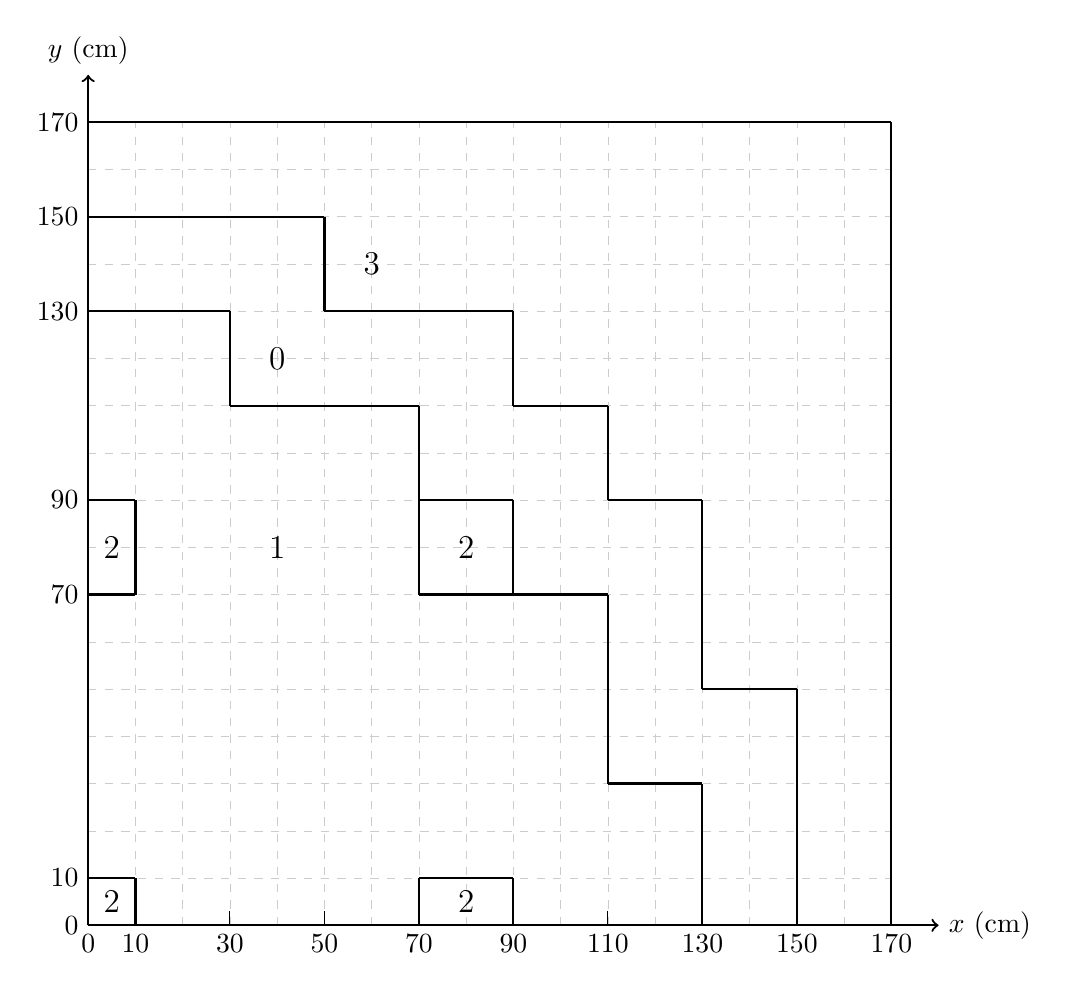
\begin{tikzpicture}[scale=.6]
\begin{scope}<->;
% GRID
 \draw[step=1.0,gray,very thin, dashed,opacity=0.4] (0.0,0.0) grid (17.0, 17.0); 
  
% AXES
  \draw[black, thick, ->] (0, 0) -- (18,  0) node[right] {$x$ (cm)};
  \draw[black, thick, ->] (0, 0) -- ( 0, 18) node[above] {$y$ (cm)};

% Material 3 regions
  \draw[black, thick] (  0.0, 17.0) -- (17.0, 17.0);
  \draw[black, thick] (  17.0, 17.0) -- (17.0, 0.0);  
  \node[font=\large] at (6.0, 14.0) {3};

% Material 0 regions
  \draw[black, thick] (  0.0, 15.0) -- (5.0, 15.0);
  \draw[black, thick] (  5.0, 15.0) -- (5.0, 13.0);  
  \draw[black, thick] (  5.0, 13.0) -- (9.0, 13.0);
  \draw[black, thick] (  9.0, 13.0) -- (9.0, 11.0);
  \draw[black, thick] (  9.0, 11.0) -- (11.0, 11.0); 
  \draw[black, thick] (  11.0, 11.0) -- (11.0, 9.0); 
  \draw[black, thick] (  11.0, 9.0) -- (13.0, 9.0); 
  \draw[black, thick] (  13.0, 9.0) -- (13.0, 5.0);
  \draw[black, thick] (  15.0, 5.0) -- (13.0, 5.0);
  \draw[black, thick] (  15.0, 5.0) -- (15.0, 0.0);
  \node[font=\large] at (4.0, 12.0) {0};

% Material 1 regions
  \draw[black, thick] (  0.0, 13.0) -- (3.0, 13.0);
  \draw[black, thick] (  3.0, 13.0) -- (3.0, 11.0);  
  \draw[black, thick] (  3.0, 11.0) -- (7.0, 11.0);
  \draw[black, thick] (  7.0, 11.0) -- (7.0, 7.0);
  \draw[black, thick] (  7.0, 7.0) -- (11.0, 7.0); 
  \draw[black, thick] (  11.0, 7.0) -- (11.0, 3.0);  
  \draw[black, thick] (  11.0, 3.0) -- (13.0, 3.0);  
  \draw[black, thick] (  13.0, 3.0) -- (13.0, 0.0);  
  \node[font=\large] at (4.0, 8.0) {1};

% Material 2 regions
  \draw[black, thick] (  0.0, 0.0) -- (0.0, 1.0);
  \draw[black, thick] (  1.0, 1.0) -- (1.0, 0.0);  
  \draw[black, thick] (  0.0, 1.0) -- (1.0, 1.0);
  \node[font=\large] at (0.5, 0.5) {2};  
  
  \draw[black, thick] (  0.0, 7.0) -- (1.0, 7.0); 
  \draw[black, thick] (  1.0, 7.0) -- (1.0, 9.0);  
  \draw[black, thick] (  1.0, 9.0) -- (0.0, 9.0);  
  \node[font=\large] at (0.5, 8.0) {2};  
  
  
  \draw[black, thick] (  7.0, 7.0) -- (9.0, 7.0);  
  \draw[black, thick] (  9.0, 7.0) -- (9.0, 9.0);  
  \draw[black, thick] (  9.0, 9.0) -- (7.0, 9.0);  
  \node[font=\large] at (8.0, 8.0) {2};

  \draw[black, thick] (  7.0, 0.0) -- (9.0, 0.0);
  \draw[black, thick] (  9.0, 0.0) -- (9.0, 1.0);
  \draw[black, thick] (  9.0, 1.0) -- (7.0, 1.0);
  \draw[black, thick] (  7.0, 1.0) -- (7.0, 0.0);
  \node[font=\large] at (8.0, 0.5) {2}; 
 
% ticks
  \foreach \x/\xtext in {0, 10, 30, 50, 70, 90, 110, 130, 150, 170}
      \draw[black,xshift=0.1*\x cm] (0,.3) -- (0,0) node[below] {$\xtext$};
  \foreach \y/\ytext in {0, 10, 70, 90, 130, 150, 170}
      \draw[black,yshift=0.1*\y cm] (.3,0) -- (0,0) node[left] {$\ytext$};

\end{scope}
\end{tikzpicture}
\caption{Geometry as modeled for the IAEA 2-D diffusion benchmark.  Material properties can be found in the benchmark documentation.  Materials 0 and 1 are fuel, material 2 represents control, while material 3 represents the outer reflector.}
\label{fig:iaea2d}
\end{figure*}

The mesh-center, finite-volume approximation was employed on a uniform, 45 $\times$ 45 spatial mesh.
The discrete ordinates transport code DETRAN was used to generate the explicit system matrix $\mathbf{A}$.
Upon discretization, the entire set of equations was cast in terms of the fission source density, i.e., $\mathbf{f} = \nu\Sigma_{f1}\phi_1(\mathbf{r}) + \nu\Sigma_{f2}\phi_2(\mathbf{r})$, which results in a $2025 \times 2025$ operator. 
Hence, problem(1) is not large, but it proved to be a valuable test case for the method, and, therefore, ensured a reasonable computing time while debugging the code.

%Note that the eigenvalue is typically updated by fission rate.
%At the time of the study, the in-house transport solver used the ratio of fluxes for the eigenvalue update.
%However, the code has since been updated to use the ratio of fission densities, and found a negligible difference in results.

All calculations were initialized with a vector in which each element was sampled from the uniform distribution $U[0, 1]$. 
This randomized starting vector helps to ensure that all eigenmodes can be present.
A formal sensitivity study was not performed to understand how this initial guess impacts the algorithm performance, but scoping studies suggest there is little impact on the number of iterations required for any particular algorithm.
In this case, a reference solution was computed using the implicitly-restarted Arnoldi method as implemented in SciPy \cite{scipy}.
All DMD calculations were performed using the Python package {\tt PyDMD} \cite{pydmd}.

\subsection{Test problem for DMD-FPM(n)}

To illustrate the performance of this method, a simple 1-D test problem was designed to resemble a slab BWR core.
This testing case was adapted from previous, transport applications from \citet{rahnema_generalized_2008}. 
The geometry of the 2-group BWR test case is shown in \FIG{fig:BWRconfig}.
\begin{figure*}[htb!]
    \centering
    \begin{minipage}[c]{\textwidth}
        \centering
        \includestandalone[mode=buildnew, width=0.85\linewidth]{tex/figures/core1}
    \end{minipage}
    \begin{minipage}[c]{\textwidth}
        \centering
        \includestandalone[mode=buildnew, width=0.3\linewidth]{tex/figures/assemblies}
    \end{minipage}
    \begin{minipage}[c]{\textwidth}
        \centering
        \includestandalone[mode=buildnew, width=0.7\linewidth]{tex/figures/core_materials}
    \end{minipage}
    \caption{Configuration for the BWR Test Problem}
    \label{fig:BWRconfig}
\end{figure*}

This core configuration had two unique assemblies.  
Three fuel types were used, including  4.5 \% enriched $UO_2$ , 2.5\% enriched $UO_2$ , and 4.5 \% enriched $UO_2$ with 5 wt\% $Gd_2O_3$.
Fuel pins for this problem were 3.2512 cm thick with 1.1176 cm of moderator on each side.
The baseline pincell discretization consisted of 18 mesh cells of fuel enclosed by six mesh cells of moderator;therefore, each pincell contained 30 mesh points.
Boundary conditions on both sides for this case were vacuum.

The final test problem was the well-studied 2-D C5G7 benchmark \cite{oecd_nuclear_energy_agency_benchmark_2003}, which was used to verify the performance of algorithm for multi-dimensional problems.
The configuration of the benchmark was adapted from \citet{reed_2015}.
The configuration of a quarter core contains four fuel-pin assemblies and five moderator assemblies as shown in \FIGURE{fig:C5G7_config}.
Each fuel assembly used 17 $\times$ 17 individual pincells, and the geometry of a $UO_2$ assembly is shown in \FIG{fig:UO2_config}, while that of a MOX assembly is shown in \FIG{fig:MOX_config}.
Here, each pincell is discretized on a 7$\times$7 Cartesian mesh.
The dimensions are shown in \FIG{fig:MOX_config}.
\begin{figure*}[htb]
    \centering
    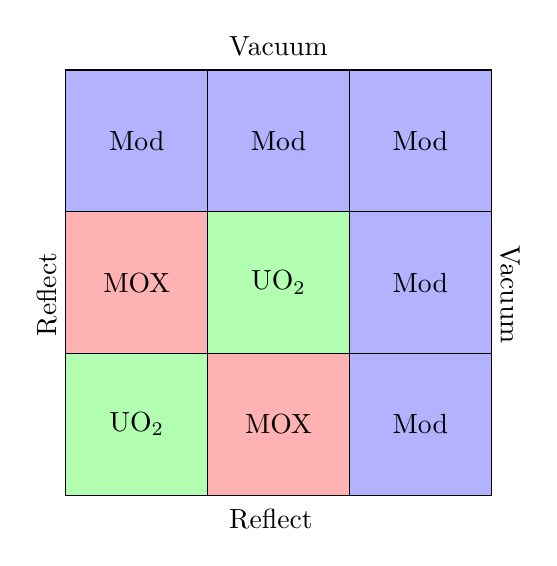
\begin{tikzpicture}[scale=0.6, every node/.style={scale=1}]
        \filldraw[xshift=6 cm, yshift=0 cm, fill=blue!30!white, draw=black] 
        (0, 0) rectangle (3,3) node[pos=.5] {Mod};
        \filldraw[xshift=6 cm, yshift=3 cm, fill=blue!30!white, draw=black] 
        (0, 0) rectangle (3,3) node[pos=.5] {Mod};
        \filldraw[xshift=6 cm, yshift=6 cm, fill=blue!30!white, draw=black] 
        (0, 0) rectangle (3,3) node[pos=.5] {Mod};
        \filldraw[xshift=3 cm, yshift=6 cm, fill=blue!30!white, draw=black] 
        (0, 0) rectangle (3,3) node[pos=.5] {Mod};
        \filldraw[xshift=0 cm, yshift=6 cm, fill=blue!30!white, draw=black] 
        (0, 0) rectangle (3,3) node[pos=.5] {Mod};
        \filldraw[xshift=0 cm, yshift=0 cm, fill=green!30!white, draw=black] 
        (0, 0) rectangle (3,3) node[pos=.5] {UO$_2$};
        \filldraw[xshift=3 cm, yshift=3 cm, fill=green!30!white, draw=black] 
        (0, 0) rectangle (3,3) node[pos=.5] {UO$_2$};
        \filldraw[xshift=3 cm, yshift=0 cm, fill=red!30!white, draw=black] 
        (0, 0) rectangle (3,3) node[pos=.5] {MOX};
        \filldraw[xshift=0 cm, yshift=3 cm, fill=red!30!white, draw=black] 
        (0, 0) rectangle (3,3) node[pos=.5] {MOX};
        \draw[xshift=9cm,yshift=4.25cm] node[right] 
        {\rotatebox{-90}{Vacuum}};
        \draw[yshift=4.25cm] node[left] {\rotatebox{90}{Reflect}};
        \draw[xshift=3.25cm,yshift=9.5cm] node[right] {{Vacuum}};
        \draw[xshift=3.25cm, yshift=-.5cm] node[right] {{Reflect}};
    \end{tikzpicture}
    \caption{Configuration for the C5G7 benchmark.  Each square represents the area of a 
             $17\times17$ pin assembly}
    \label{fig:C5G7_config}
\end{figure*}

\begin{figure*}[htb]
    \centering
    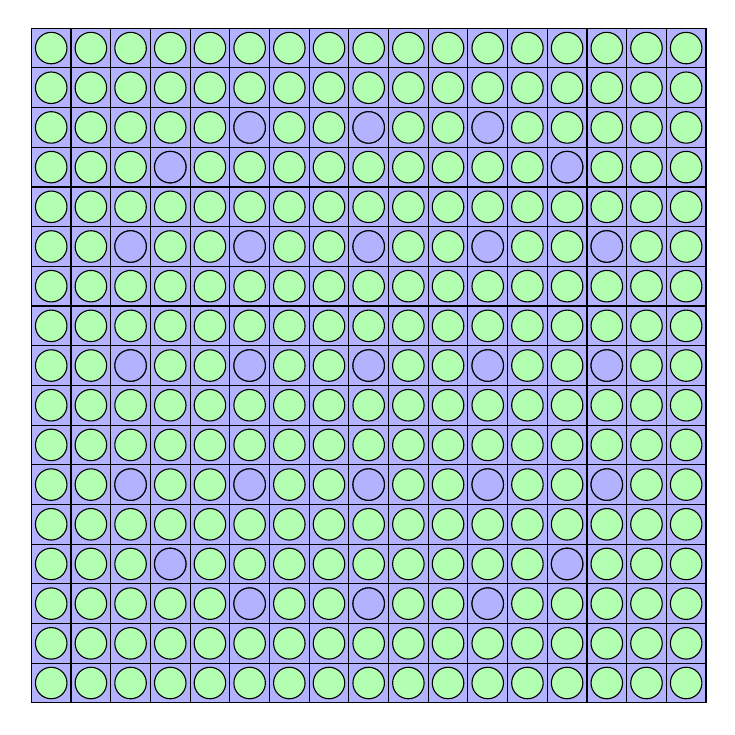
\begin{tikzpicture}[scale=0.4, every node/.style={scale=1}]
        \foreach \x in {0,1.26,...,20.16}
        \foreach \y in {0,1.26,...,20.16}
        \filldraw[xshift=\x cm, yshift=\y cm, fill=blue!30!white, 
        draw=black] (0, 0) rectangle (1.26,1.26) node[pos=.5] {};
        \foreach \x in {0,1.26,...,20.16}
        \foreach \y in {0,1.26,...,20.16}
        \filldraw[xshift=\x cm, yshift=\y cm, fill=green!30!white, 
        draw=black] (.63,.63) circle (.5) node[pos=.5] {};
        \foreach \x in {5*1.26, 8*1.26, 11*1.26}
        \foreach \y in {2*1.26, 14*1.26}
        \filldraw[xshift=\x cm, yshift=\y cm, fill=blue!30!white, 
        draw=black] (.63,.63) circle (.5) node[pos=.5] {};
        \foreach \x in {3*1.26, 13*1.26}
        \foreach \y in {3*1.26, 13*1.26}
        \filldraw[xshift=\x cm, yshift=\y cm, fill=blue!30!white, 
        draw=black] (.63,.63) circle (.5) node[pos=.5] {};
        \foreach \x in {2*1.26, 5*1.26, 8*1.26, 11*1.26, 14*1.26}
        \foreach \y in {5*1.26, 8*1.26, 11*1.26}
        \filldraw[xshift=\x cm, yshift=\y cm, fill=blue!30!white, 
        draw=black] (.63,.63) circle (.5) node[pos=.5] {};
    \end{tikzpicture}
    \caption{Configuration for a UO$_2$ fuel bundle.  The green represents a 
             UO$_2$ pincell, while the blue represents a guide tube modeled as 
             a pincell filled with moderator}
    \label{fig:UO2_config}
\end{figure*}

\begin{figure*}[htb]
    \centering
    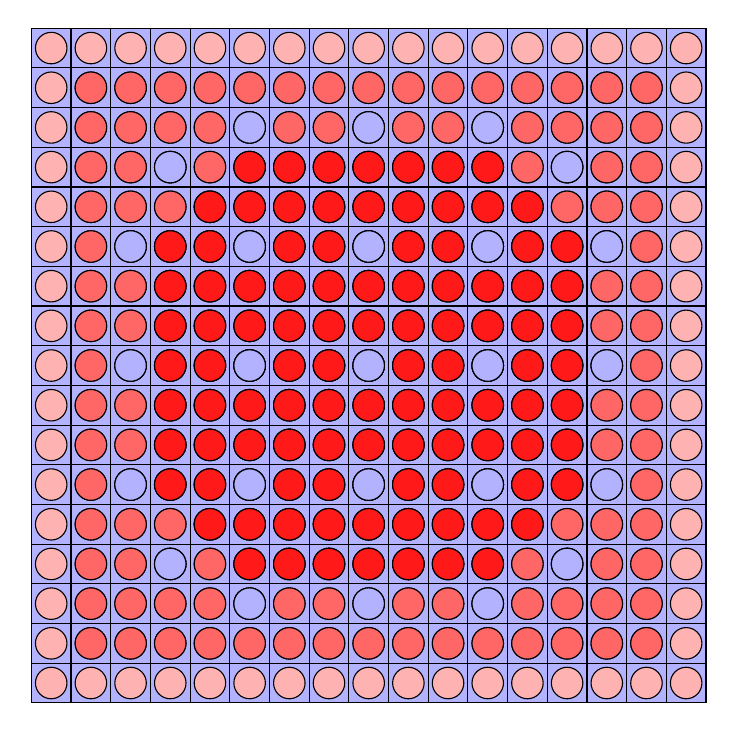
\begin{tikzpicture}[scale=0.4, every node/.style={scale=1}]
        \foreach \x in {0,1.26,...,20.16}
        \foreach \y in {0,1.26,...,20.16}
        \filldraw[xshift=\x cm, yshift=\y cm, fill=blue!30!white, 
        draw=black] (0, 0) rectangle (1.26,1.26) node[pos=.5] {};
        \foreach \x in {0,1.26,...,20.16}
        \foreach \y in {0,1.26,...,20.16}
        \filldraw[xshift=\x cm, yshift=\y cm, fill=red!30!white, draw=black] 
        (.63,.63) circle (.5) node[pos=.5] {};
        \foreach \x in {1.26,2.52,...,20.16}
        \foreach \y in {1.26,2.52,...,20.16}
        \filldraw[xshift=\x cm, yshift=\y cm, fill=red!60!white, draw=black] 
        (.63,.63) circle (.5) node[pos=.5] {};
        \foreach \x in {5*1.26,6*1.26,7*1.26,8*1.26,9*1.26,10*1.26,11*1.26}
        \foreach \y in {3*1.26,13*1.26}
        \filldraw[xshift=\x cm, yshift=\y cm, fill=red!90!white, draw=black] 
        (.63,.63) circle (.5) node[pos=.5] {};
        \foreach \x in 
        {4*1.26,5*1.26,6*1.26,7*1.26,8*1.26,9*1.26,10*1.26,11*1.26,12*1.26}
        \foreach \y in {4*1.26,12*1.26}
        \filldraw[xshift=\x cm, yshift=\y cm, fill=red!90!white, draw=black] 
        (.63,.63) circle (.5) node[pos=.5] {};
        \foreach \x in {3.78,5.04,...,16.38}
        \foreach \y in {6.3,7.56,...,15.04}
        \filldraw[xshift=\x cm, yshift=\y cm, fill=red!90!white, draw=black] 
        (.63,.63) circle (.5) node[pos=.5] {};
        \foreach \x in {5*1.26, 8*1.26, 11*1.26}
        \foreach \y in {2*1.26, 14*1.26}
        \filldraw[xshift=\x cm, yshift=\y cm, fill=blue!30!white, 
        draw=black] (.63,.63) circle (.5) node[pos=.5] {};
        \foreach \x in {3*1.26, 13*1.26}
        \foreach \y in {3*1.26, 13*1.26}
        \filldraw[xshift=\x cm, yshift=\y cm, fill=blue!30!white, 
        draw=black] (.63,.63) circle (.5) node[pos=.5] {};
        \foreach \x in {2*1.26, 5*1.26, 8*1.26, 11*1.26, 14*1.26}
        \foreach \y in {5*1.26, 8*1.26, 11*1.26}
        \filldraw[xshift=\x cm, yshift=\y cm, fill=blue!30!white, 
        draw=black] (.63,.63) circle (.5) node[pos=.5] {};
    \end{tikzpicture}
    \caption{Configuration for a MOX bundle.  The light red represents 4.3\% MOX 
             fuel, the medium red represents 7.0 \% MOX fuel, and the dark red 
             represents 8.7\% MOX fuel.  The blue represents moderator (i.e.,  
             light water)}
    \label{fig:MOX_config}
\end{figure*}



\begin{figure*}[htb]
    \centering
    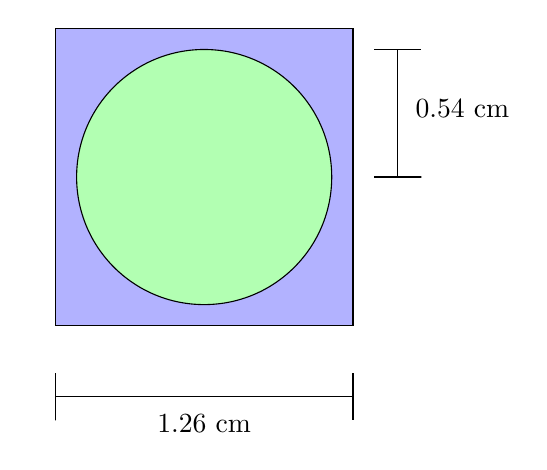
\begin{tikzpicture}[scale=3, every node/.style={scale=1}]
        \filldraw[xshift=0 cm, yshift=0 cm, fill=blue!30!white, draw=black] 
        (0, 0) rectangle (1.26,1.26) node[pos=.5] {};
        \filldraw[xshift=0 cm, yshift=0 cm, fill=green!30!white, draw=black] 
        (.63,.63) circle (.54) node[pos=.5] {};
        \draw (0,-.2) -- (0,-.4) -- (0,-.30) -- (0.63,-.3) node[below=0.1cm] 
        {1.26 cm} -- (1.26,-.30) -- (1.26,-.2) -- (1.26, -.4);
        \draw (1.35,.63) -- (1.55,.63) -- (1.45,.63) -- (1.45,.92) 
        node[right=0.1cm] {0.54 cm} -- (1.45,1.17) -- (1.35,1.17) -- (1.55, 
        1.17);
    \end{tikzpicture}
    \caption{Configuration for pincell.  The circular fuel element had a 
             radius of 0.54 cm and was homogenized with cladding for this 
             model.}
    \label{fig:pin_cell_config}
\end{figure*}
Here, the neutron transport equation for both 1-D and 2-D problems are solved by the discrete ordinates method, and all DMD calculations were performed using the PyDMD \cite{pydmd}.
An S4 Gauss-Legendre quadrature was used with the diamond difference approximation.
The reference eigenvalue and eigenvector were computed using full power iteration (i.e., fully converging the scattering source at each eigen iteration).

\section{Results for DMD-PM(n)}
As mentioned in the previous chapters, the major cost of the power method is from solving $\mathbf{Ax =b}$.
In this case, the computational time is proportional to the number of iterations.
Thus, the number of iterations is used as the indicator of computational cost in the following comparisons.

\subsection{Skipping Ahead with DMD-PM(n)}
As a first test of the method of DMD-PM($n$), the goal was to verify that DMD predicted eigenmodes prediction are closer to converged solutions.
A series of $n$ power iterations was performed to generate the snapshots, then the dominant eigenmode
was reconstructed as a function of iteration using \EQ{eq:dmd_predict}.
The absolute error with respect to the reference eigenmode was computed as the euclidean norm of the differences, or
\begin{equation}
 ||\mathbf{e}|| =  ||\mathbf{x}^{*}_i-\mathbf{x}_{ref}||_2   \, .
 \label{eq:error}
\end{equation}
The results shown in \FIGURE{fig:skipahead} are predicted using different number $n$ of snapshots where ``time'' is increasing.
Shown in parentheses is the number of equivalent power iterations to which the final, saturated error in the DMD prediction corresponds.
For example, application of 30 power iterations leads to a DMD surrogate that can predict an eigenmode with an accuracy equal to 149 power iterations, a substantial skip ahead in the number of iterations.

\begin{figure}[htb]%t=top, b=bottom, h=here
    \centering
    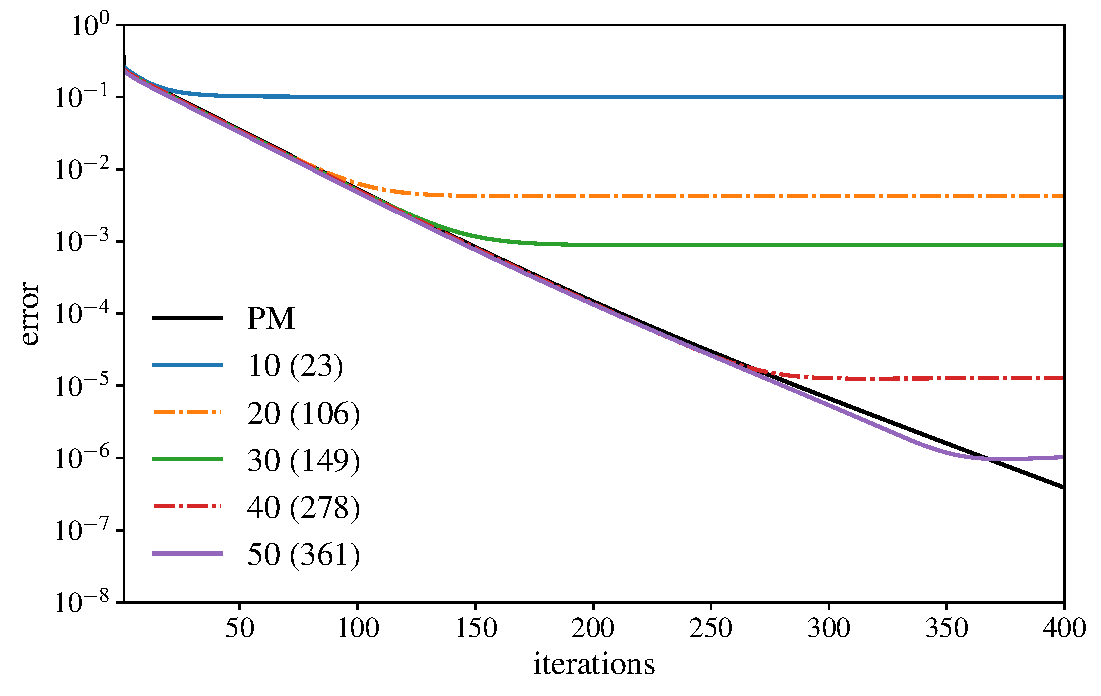
\includegraphics[height=4.0in]{tex/figures/skipahead.pdf}
   \caption{Error in the DMD-predicted, dominant eigenmode as a function of iteration.  The legend shows the number of power iterations $n$ used to construct the surrogate, and in parentheses is the effective number of power iterations the DMD surrogate can produce.}
  \label{fig:skipahead}
\end{figure}

The error shown in \FIGURE{fig:skipahead} approaches an asymptotic, lower bound as predictions are made beyond the number of power iterations used to generate the DMD surrogate.
As expected, a larger snapshots matrix can provide more information for learning the function and mapping a more accurate output.
Note that the final result reaching the lower bound here is very closed to the direct solution predicted by only the dominant DMD modes $\mathbf{\Phi_0}$, which demonstrate that our modified \EQUATION{eq:f_mode} can produce results with the same level of accuracy.

\subsection{Application of Restarted DMD-PM(n)}
As mentioned in \CHAPTER{chapter:DMD-PM}, the DMD-PM($n$) should restart from a set of snapshots multiple times until the solution converges.
To test the performance of the iterative application of the DMD-PM($n$) scheme, we used a fixed number $n$ at every restart to research the convergence.  
The results are shown in \FIGURE{fig:dmdpi_semilog}, which also includes the error for the unaccelerated PM and the Arnoldi method.
Here, the Arnoldi method was used without restarts. 
The results shown for the Arnoldi method are as a function of the size of the subspace used.

Note that the restart value for Restarted DMD-PM($n$) were selected as same as the skip ahead test.
Although a larger restart value can often yield a better acceleration, storing a larger number of snapshots uses more memory and requires more operations during the SVD decompostion.
Here, we consider the each DMD extrapolation process as an iteration on the horizontal, and, therefore, the final end points do not match exactly.

\begin{figure}[htb]%t=top, b=bottom, h=here
    \centering
    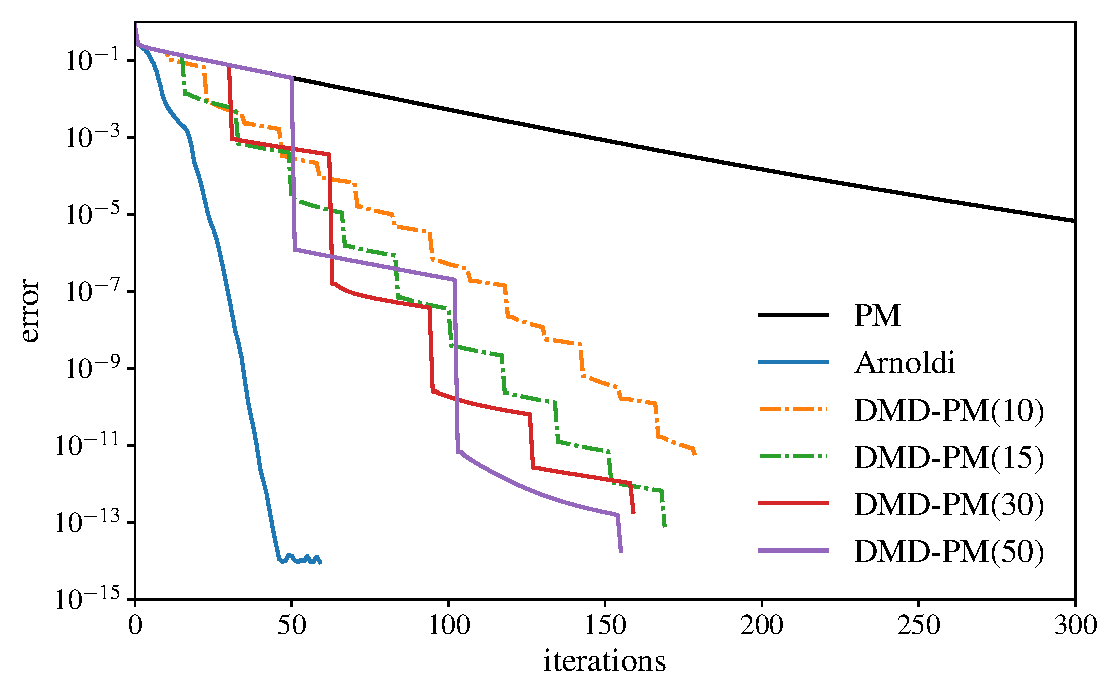
\includegraphics[height=4.0in]{tex/figures/dmdpi_semilog.pdf}
    \caption{The error in the predicted eigenmode for DMD-PM($n$), where $n$ is the number of power iterations performed.  Errors are also included for the power method (PM) and Arnoldi's method.}
    \label{fig:dmdpi_semilog}
\end{figure}

In this case, a tolerance of $10^{-14}$ is used as the tolerance for convergence.
For reference, approximately 800 unaccelerated power iterations are required to reach this error.
Ignoring the cost from DMD, the best DMD-PM($50$) only required around 150 iterations to reach the same error, thus providing (5$\times$) speedup compared to unaccelerated power iterations.

On the other hand, there is a significant performance difference between DMD-PM($n$) and the Arnoldi method, which is also expected.
The Arnoldi method only requires around 40 iterations to converge.
The Arnoldi method is based on a subspace that undergoes continuous orthonormalization, which produces a better-conditioned and, likely, richer basis than can be produced by successive application of $\mathbf{A}$ to a single vector.
Consequently, it is inapplicable when the explicit form of $\mathbf{A}$ is not available.  

\section{Results for DMD-FPM(n)}
As mentioned in the \CHAPTER{chapter:PM}, the flattened PM eliminates the inner iterations and only apply one transport sweep each iteration.
Therefore, we used number of sweeps as the measure for the total computational cost, which is equivalent to number of iterations.
Two similar tests on different geometries are conducted and solved for a variety of restart values $n$ to study the optimum condition.
The reference solutions were computed using full power method (i.e.,fully converging the scattering source at each eigen iteration).
The error is defined as same as \EQUATION{eq:error}, and the tolerance of convergence is set as $10^{-8}$.

\subsection{DMD-FPM(n) for 1D BWR Test Problem}

To compare performance, the generalized $k-$eigenvalue problem was solved first by flattened power iteration, which used 3445 transport sweeps for this BWR problem.
The best DMD-FPM($n$) algorithm used 40 snapshots, and required approximately 270 transport sweeps, thus providing more than an order of magnitude reduction in the computational cost.

\begin{figure}[htb]%t=top, b=bottom, h=here
    \centering
    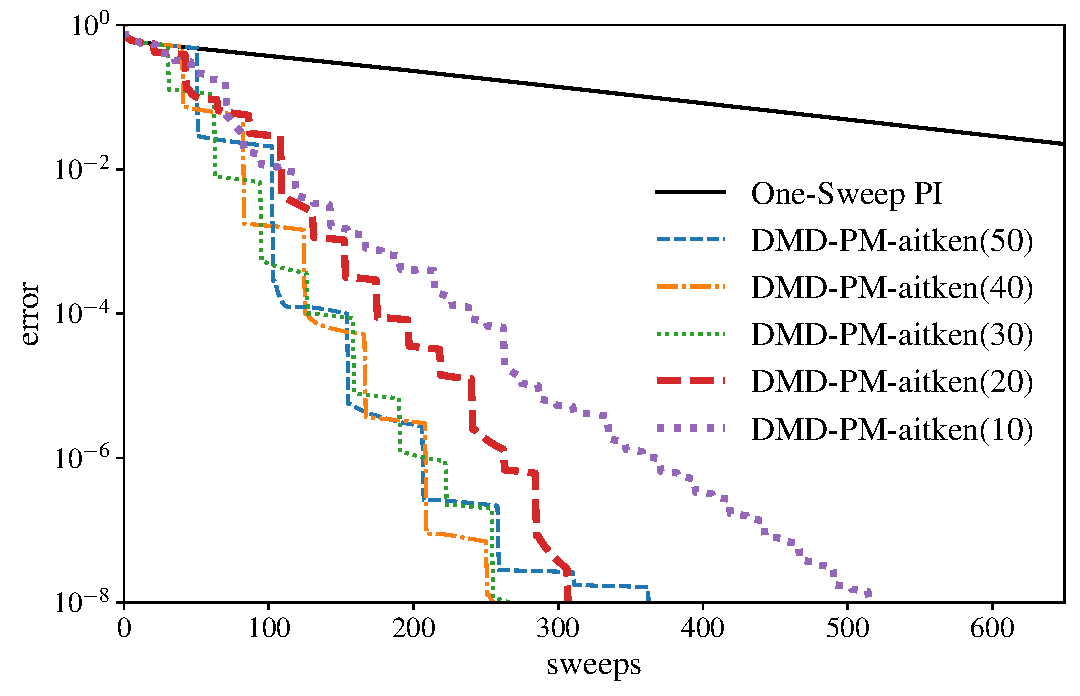
\includegraphics[height=4.0in]{tex/figures/dmd_ospi_semilog_1d.pdf}
    \caption{The absolute error in the predicted eigenmode for DMD-PM-aitken(n) for the 1D BWR problem, where n is the number of transport sweeps performed.}
    \label{fig:DMD-FPM_1d}
\end{figure}

This case shows that using a larger number of snapshots cannot promise a faster convergence for DMD-FPM($n$).
The reason might be the error remaining from dismatched eigenvalues.

\subsection{DMD-FPM(n) for 2D C5G7 Test Problem}

Similar the 1-D results, the results of C5G7 2-D benchmark also show that the best condition of DMD-FPM($n$) algorithm has significant speedup compared to flattened power iteration, which required 351 transport sweep to reduce error to $1e-8$ while using 30 snapshots each restart.
For reference, approximately 1570 unaccelerated flattened power sweeps are required for this problem to be fully converged.
As expected in this case, a small increase in error may be observed more obviously for each application of DMD-FPM($n$) due to the previously discussed eigenvalue error.
And the best case is not using the most number of snapshots, though the difference of sweeps is relatively small.

\begin{figure}[htb]%t=top, b=bottom, h=here
    \centering
    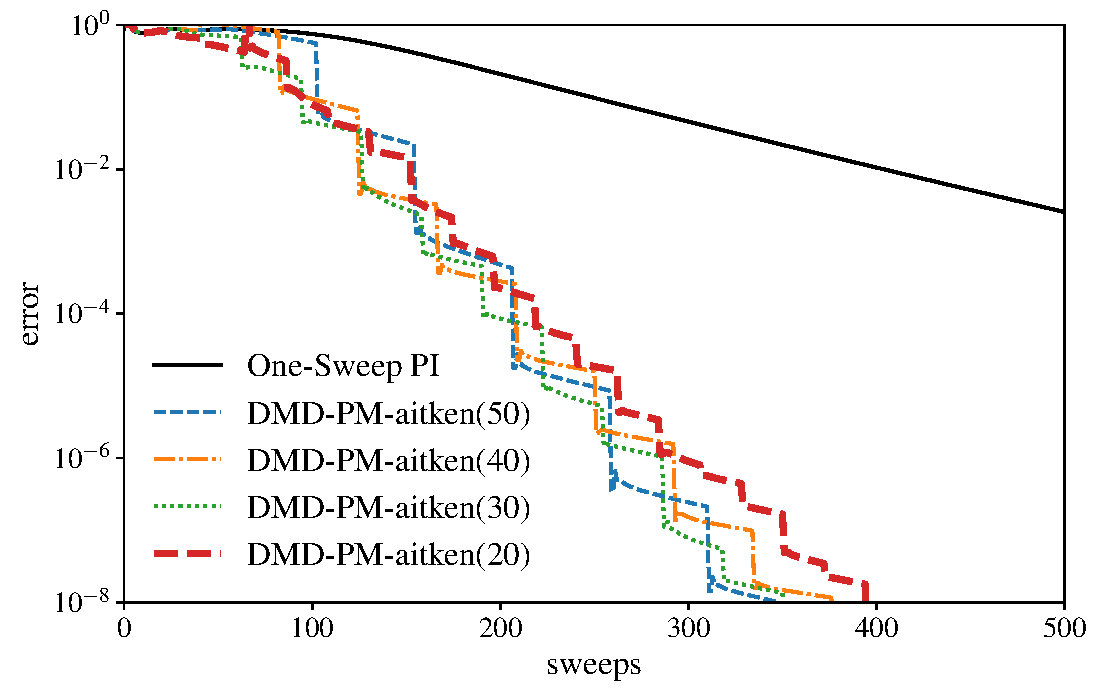
\includegraphics[height=4.0in]{tex/figures/dmd_ospi_semilog_c5g7.pdf}
    \caption{The absolute error in the predicted eigenmode for DMD-PM-Aitken(n) for the 2D C5G7 problem, where n is the number of transport sweeps performed.}
    \label{fig:DMD-FPM_2d}
\end{figure}

Using DMD too frequently (i.e., small $n$) might produce a large numerical error from SVD decomposition, the error increase many level of magnitude from DMD.
This is the reason why DMD-FPM($10$) did not reduce the error to within the target range.
The number of transport sweeps required to reach a tolerance of $10^{-8}$ are shown in \TAB{tab:widetable}.

\begin{table*}[htb]
  \centering
  \small
  \caption{Number of transport sweep}
  \begin{tabular}{lllllllll}\toprule
      & FPM  & DMD-FPM(10)& DMD-FPM(20)& DMD-FPM(30)& DMD-FPM(40)& DMD-FPM(50)
\\ \midrule
$BWR$  & 3444 & 515 & 307 & 267 & 256 & 363
\\
$C5G7$  & 1570  & N/A & 395 & 351 & 377 & 395
\\
\bottomrule
\end{tabular}
  \label{tab:widetable}
\end{table*}

% +--------------------------------------------------------------------+
% | Sample Chapter 2
% +--------------------------------------------------------------------+

\cleardoublepage

% +--------------------------------------------------------------------+
% | Replace "This is Chapter 2" below with the title of your chapter.
% | LaTeX will automatically number the chapters.                      
% +--------------------------------------------------------------------+

\chapter{Conclusions and Future Work}
\label{chapter:conclusion}
\section{Summary}
First, the principal objective of this thesis was to accurately estimate fundamental eigenmodes by DMD to accelerate the power method and flattened power method for multigroup neutron transport/diffusion problems.
Although DMD is a useful tool for extracting information from data, often it can only be applied on the snapshots from the time-dependent dynamic systems.
In \CHAPTER{chapter:DMD-FPM(n)}, we have presented a new scheme for identifying fundamental eigenvector by a improved DMD algorithm using only the dominant DMD modes, which allows us to correct the solution by a more accurate estimation of the steady solution. 
This restarted version DMD-PM($n$) can be applied repeatedly to accelerate the power method.

Flattened iterations update the fission and scattering source at the same time and reduced the total number of transport sweeps in practice, which has been widely used as an  more efficient alternative of the power method.
Therefore, we also explored a similar scheme DMD-FPM($n$) to improve the convergence rate of the flattened power method, 
Because the eigenvalue cannot be computed by the eigenvector from flattened operator, the Aitken method is employed to extrapolate the eigenvalues corresponding to the DMD prediction.

To base the comparison, three test problems were conducted, which include (1) a 2-D, IAEA diffusion benchmark, (2) a 1-D, 70-pin BWR core model, and (3) the 2-D C5G7 benchmark.
Through all the numerical examples, we demonstrated that both acceleration schemes provide promising speedup. 
The choice of number of snapshots to DMD greatly impacts the effectiveness, the DMD-PM(50) case used only 25\% number of power iterations to solve the IAEA diffusion problem.
This scheme has also been used to produce a approximation of higher-order modes.
Unfortunately, the accuracy of the two higher-order modes are not as good as the dominant mode.
Although DMD-PM($n$) might not be competitive with other advance acceleration schemes (e.g., the Arnold method), there do exist applications for which access to iterates is only available in a postprocessing sense.
As can be expected, DMD-FPM($n$) provided approximately a 5x$-$10x speedup for the two cases studied.
However, the failure of DMD-FPM($10$) in solving C5G7 case indicate that DMD might produce a large numerical error from SVD when the results are closed to the steady-state solution, because the snapshots are linearly dependent.
In this case, the DMD should be stopped, and using only the power or flattened power method to reduce the error to within the target range.

\section{Future Research}
In this section, we describe the future direction and substantial value of using these methods in other areas.
While these results are promising, the performance of both schemes are not expected to outperform some other popular methods, such as the generalized Davidson method\cite{hamilton2011numerical} and coarse-mesh finite difference\cite{smith_1983}.
In reactor analysis, the use of stochastic methods, such as the famous Monte Carlo simulations, is widespread.
Following this thesis, application of DMD-PM($n$) and DMD-FPM($n$) may be able to accelerate Monte Carlo eigenvalue problems for convergence by regressing the distribution tendency of neutron population from DMD modes.
In this way, only a small size of neutron populations are sufficient to generate snapshots and extract information, which might be comparable to the other acceleration methods.

Although Aitken extrapolation could estimate the eigenvalues corresponding to DMD responses, errors still exist at almost every restart point, and, therefore, reducing the desired accuracy. 
More work can also be done in the future to compute the corresponding eigenvalues, which can improve the performance while a great amount of restarted process is required in the large scale systems.


% +--------------------------------------------------------------------+
% | Uncomment the lines below to add additional chapters.
% +--------------------------------------------------------------------+

%\cleardoublepage

\chapter{Dynamic Mode Decomposition}
\label{chapter:DMD-PM}

Before introducing how to use dynamic mode decomposition to accelerate the power and flattened power methods, we will first review the details of DMD.
As mentioned in Chapter 1, the details of DMD are different based on the application.
However, most of these varieties share a familiar, straightforward frame. 
Here, the most widely-used variant (called ``standard DMD'' here) will be shown as an example to represent the algorithm.

To start, first consider the generic, dynamic problem defined by 
\begin{equation}
  \frac{d{\mathbf{x}}}{dt}=\mathbf{f}(\mathbf{x},t) \, ,
  \label{eq:dynamic_problem}
\end{equation}
where $\mathbf{x} \in \mathbb{R}^{n}$ is the $n$-dimensional state vector at time $t$. 
With sufficiently small steps in time, the evolution of  $\mathbf{x}$ can be well approximated by a relationship of the form 
\begin{equation}
 \frac{d{\mathbf{x}}(t)}{dt}=\mathcal{A}\mathbf{x} \, ,
 \label{eq:linearized_model}
\end{equation}
where the evolution operator $\mathcal{A}$ may be unknown and can be considered a ``black-box'' system.
However, one can obtain the system state $\mathbf{x}_n$ at different times, which are then stacked as the past and future snapshot matrices $ \mathbf{X}_0$ and $ \mathbf{X}_1$, i.e., 
\begin{equation}
\label{eq:past_data}
\mathbf{X_0}=\left[ \mathbf{x}_0, \mathbf{x}_1, \ldots, \mathbf{x}_{m-1} \right] \, ,
\end{equation}
and
\begin{equation}
\label{eq:future_data}
\mathbf{X_1}=\left[ \mathbf{x}_1, \mathbf{x}_2, \ldots, \mathbf{x}_{m} \right] \, .
\end{equation}

Suppose $\mathbf{A}$ is the discrete-time approximation of the mapping operator $\mathcal{A}$:
\begin{equation}
\label{eq:A}
\mathbf{A} = e^{\mathcal{A} \Delta t} \, .
\end{equation}
Then,
\begin{equation}
\label{eq:x0x1}
\mathbf{x}_{k+1} = \mathbf{A} \mathbf{x}_{k}, \quad \quad k = 0,1,...,\, .
\end{equation}
In general, the approximate operator $\mathbf{A}$ not reproduce the $\mathbf{x}_i$ exactly, but a ``best'' approximation can be formed in a least-squares or minimum-norm sense by solving
\begin{equation}
\label{eq:least}
\mathbf{A} =  \underset{\mathbf{A}}{argmin} ||\mathbf{X}_1 - \mathbf{A} \mathbf{X}_0||_F \, .
\end{equation}
Thus, the best-fit operator $\mathbf{A}$ is formally given by 
\begin{equation}
\label{eq:fullA}
A = \mathbf{X}_1 \mathbf{X}_0^{\dagger} \, ,
\end{equation}
where $\mathbf{X}_0^{\dagger}$ is the Moore-Penrose generalized inverse of $\mathbf{X}_1$.
It is possible (and typical) to use SVD factorization to find the inverse of $\mathbf{X}_1$ by
\begin{equation}
\label{eq:svd}
\mathbf{X}_0 = \mathbf{U} \bm{\Sigma} \mathbf{V}^{*} \rightarrow \mathbf{X}_0^{\dagger} = \mathbf{V} \bm{\Sigma}^{-1} \mathbf{U}^* \, ,
\end{equation}
where $\mathbf{U} \in \mathbb{C}^{m\times n}$, $\mathbf{V} \in \mathbb{C}^{n\times n}$, $\bm{\Sigma} \in \mathbb{C}^{n\times n}$, and $*$ indicate the conjugate transposes. 

However, considering that the number of unknowns in this matrix is often large during numerical simulations, the matrix $\mathbf{A}$ is not computed explicitly.
A low-rank approximation of the original dynamic system $\mathbf{\tilde{A}}$ is formed, i.e.,
\begin{equation}
\label{eq:reduced_dmd_1}
\mathbf{\tilde{A}} =  \mathbf{U_r^* A U_r} \, .
\end{equation}
Then using \EQ{eq:fullA}, the reduced order $\mathbf{\tilde{A}}$ is defined by
\begin{equation}
\label{eq:reduced_dmd_2}
\mathbf{\tilde{A}} =  \mathbf{U_r^*} \mathbf{X_1} \mathbf{V} \bm{\Sigma}^{-1} \, .
\end{equation}
Now extract the $r$ largest eigenvalue and corresponding eigenvectors from $\mathbf{\tilde{A}}$ as the DMD modes $\boldsymbol{\Phi}$, which can be treated as the leading $r$ eigenvectors of $\mathbf{A}$.
Note that the solution of \EQ{eq:linearized_model} is $\mathbf{x}(t) = e^{\mathcal{A}t}\mathbf{x}(0)$, and $\mathbf{A}$ is a discrete-time approximation of $e^{\mathcal{A}\Delta}$, which can be applied to the initial condition using the matrix exponential to compute the solution at a particular time. 
Moreover, the discrete eigenvalues $\lambda_i$ of $\mathbf{A}$ can be used to compute the continuous eigenvalues $\omega_i= \text{log}(\lambda_i)/\Delta t$.
Subsequently, the state can be reconstructed at any time $t$ by initial condition by  
\begin{equation}
\label{eq:dmd_predict}
\vec{x}^{DMD}(t) \triangleq \sum_{i=1}^{r} \vec{\phi}_i e^{\omega_it} b_i \, ,
\end{equation}
where $\mathbf{b}=\boldsymbol{\Phi}^{\dag} \mathbf{x}_{0}$. 

The general DMD scheme is summarized as
\begin{enumerate}
\item Compute SVD decomposition of the forward snapshots matrix, i.e., $ \mathbf{X_0} = \mathbf{U_r} \boldsymbol{\Sigma_r} \mathbf{V_r^{*}}$, where r indicates the rank of matrix.
\item Compute $\mathbf{\tilde{A}}=\mathbf{U_r^{*}X_1}\mathbf{V_r}\boldsymbol{\Sigma}_{\mathbf{r}}^{-1}$, where $\mathbf{A}$ and $\mathbf{\tilde{A}}$ are similar matrices.
\item Compute the eigendecomposition $\mathbf{\tilde{A} \tilde{W}}=\boldsymbol{\Lambda}\mathbf{\tilde{W}}$.
\item Calculate the DMD modes as ${\boldsymbol{\Phi}}={\mathbf{X_2V_r}}\boldsymbol{\Sigma}_\mathbf{r}^{-1}{\mathbf{\tilde{W}}}$.
\item Predict the response by $\vec{x}^{DMD}(t) \approx \sum_{i=1}^{r} \vec{\phi}_i e^{\omega_it} b_i = \boldsymbol{\Phi}{\mathbf{diag}}(e^{\vec{\omega}t})\vec{b}$, where $\mathbf{b}=\boldsymbol{\Phi}^{\dag} \mathbf{x}_{0}$.
\end{enumerate}




%% +--------------------------------------------------------------------+
% | Sample Chapter 2
% +--------------------------------------------------------------------+

\cleardoublepage

% +--------------------------------------------------------------------+
% | Replace "This is Chapter 2" below with the title of your chapter.
% | LaTeX will automatically number the chapters.                      
% +--------------------------------------------------------------------+

\chapter{Results}
\label{makereference2}

To refer to Chapter~\ref{makereference1}, use the slash ref command
along with the "makereference" label which was assigned back at the
beginning of Chapter 1.

\section{Page Number References}
\label{makereference2.1} It is possible to refer to a specific page
number, such as page~\pageref{makereference1}.  Add a slash label
command and a unique name for each page to be referenced later in
the text.

\section{Referring to Sections Within Chapter 1}
\label{makereference2.2} It is possible to refer to sections within
a chapter.  Add a slash label command and a unique name with the
section number for each section to be referenced later in the text.
Here is an example of a figure in section~\ref{makereference1.1} and
an example of a table in section~\ref{makereference1.2}.  In
section~\ref{makereference1.3}, we looked at examples of
bibliographic citations.


% +--------------------------------------------------------------------+
% | References
% +--------------------------------------------------------------------+

% +--------------------------------------------------------------------+
% | Included for Gather Purpose only.  Do NOT uncomment the next line.
%input "tex/refs/references.bib"
% | In order for the WinEDT editor to index references correctly, it
% | has to know where the "references.bib" file resides.  This
% | command will be ignored completely by LaTeX
% |
% | WinEDT can read file path names with either "\" or "/". LaTeX,
% | however,doesn't like "\", so it's easier to store a path name
% | using forward slashes "/".
% +--------------------------------------------------------------------+

\cleardoublepage
\phantomsection

% +--------------------------------------------------------------------+
% | This template uses the BibTeX program to format references.  The
% | lines below create a separate Bibliography section and add
% | an entry for "Bibliography" to the Table of Contents.  The actual
% | data for your references (author, title, journal, date, etc.) are
% | entered in the references.bib file.  See "Citations and Bibliography"
% | for details on to creating citations and formatting references.
% +--------------------------------------------------------------------+

\addcontentsline{toc}{chapter}{Bibliography}
\bibdata{tex/refs/references}
\bibliography{tex/refs/references}

% +--------------------------------------------------------------------+
% | The following commands add the appendices  To add or delete
% | appendices, add or remove the line
% |
% |     \input{appendixX.tex}
% |
% | where "X" is the letter designation of the appendix (A, B, C,
% | etc.) You should have one \input{appendixX.tex} line and a
% | corresponding file appendixX.tex for each appendix.
% |
% |If you do not have any appendices, comment out or delete the three
% |lines below.
% +--------------------------------------------------------------------+

\appendix
%% +--------------------------------------------------------------------+
% | Appendix A Page (Optional)                                         
% +--------------------------------------------------------------------+

\cleardoublepage

\chapter{Title for This Appendix}

\label{Appendix:Key1}

Enter the content for Appendix A in the appendixA.tex file.  If you
do not have an Appendix A, see comments in the etdrtemplate.tex file
for instructions on how to remove this page.

%% +--------------------------------------------------------------------+
% | Appendix B Page (Optional)                                         
% +--------------------------------------------------------------------+

\cleardoublepage

\chapter{Title for This Appendix}
\label{Appendix:Key2}

Enter the content for Appendix B in the appendixB.tex file. If you
do not have an Appendix B, see comments in the etdrtemplate.tex file
for instructions on how to remove this page.


\end{document}

% +--------------------------------------------------------------------+
% | Template Revisions
% |
% | 9/14/06: Removed typos
% | 3/29/13: Removed hypernat package
% | 4/5/13: Changed to plain bib style
% | 5/17/13: added /cleardoublepage and /phantomsection to
% |          /bibliography to correct TOC page problem
% | 5/17/13: Fixed TOC problem with Dedication, Preface, etc.
% | 12/16/15: Added tocloft package to produce leader dots for all
% |           entries in the table of contents.
% |           Added geometry package to specify 1 inch margins.
% |           Removed unnecessary color specifications.
% |           Changed to \citep for citations.
% | 2/9/2016: Replaced \bibpunct with \setcitestyle.
% |           Changed to unsrtnat style
% |           Added natbib.pdf and Citations and Bibliography.pdf files
% | 8/3/2018: Fixed problem with incorrect page numbers for
% |           Acknowledgements, Dedication, and Preface in TOC.
% |           Removed limit on number of words in Abstract.
% +--------------------------------------------------------------------+
